\section{第1章 引言:微生物组 - 免疫检查点轴的临床需求与理论基础}\label{ux7b2c1ux7ae0-ux5f15ux8a00ux5faeux751fux7269ux7ec4---ux514dux75abux68c0ux67e5ux70b9ux8f74ux7684ux4e34ux5e8aux9700ux6c42ux4e0eux7406ux8bbaux57faux7840}

\pandocbounded{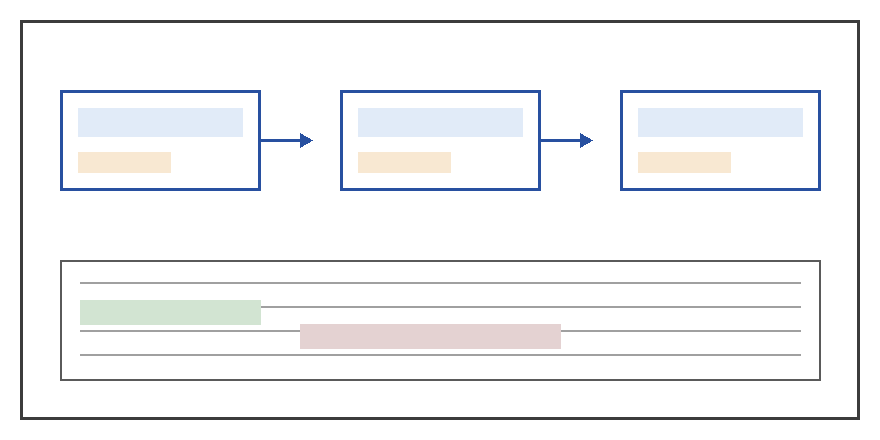
\includegraphics[keepaspectratio]{assets/FIG_06_history_demo.png}}

\textbf{图 1. 06集成fixture演示图(复用04验收样本图,非新科研制图):证据地图示意 {[}1{]}。}

(06集成fixture \(\cdot\) 引言)本节说明综述的范围与各章分工:先建立评估框架,再进入机制与调节因素,最后讨论干预与转化边界;各章安排与结语承诺一致。

\begin{quote}
本章论断:本章确立肠道微生物组作为调节实体瘤 ICI 疗效的关键系统性因子的理论地位。首先通过 ICI 疗效异质性(含超进展)及传统标志物局限阐明临床紧迫性;其次构建微生物 - 免疫 - 疗效的多维机制框架并区分证据等级;最后明确综述范围(实体瘤、ICI),排除血液瘤及非 ICI 疗法以避免概念外推错误。
\end{quote}

\subsection{1.1 免疫治疗的疗效差异与临床需求}\label{ux514dux75abux6cbbux7597ux7684ux7597ux6548ux5deeux5f02ux4e0eux4e34ux5e8aux9700ux6c42}

免疫检查点抑制剂(ICI)虽已确立为多种晚期实体瘤的标准治疗手段,但其临床获益存在显著的个体差异,部分患者不仅无法获益,甚至出现超进展(Hyperprogressive Disease, HPD)等极端负面反应。在一项纳入 187 名接受 ICI 治疗的实体瘤患者的回顾性队列中,基于肿瘤生长率变化(\(\Delta TGR \geq 2\) 倍)定义的 HPD 发生率为 10\%,且该表型与显著较差的总生存期(OS)相关,尤其在非小细胞肺癌(NSCLC)亚组中更为明显 {[}2{]}。这一现象在真实世界社区医疗环境中同样得到验证,采用仅需基线与治疗后两次影像扫描的改良定义,HPD 发生率约为 13\%,HPD 患者的中位 OS 仅为 5.5 个月,显著低于非 HPD 患者的 18.3 个月 {[}3{]}。HPD 的存在表明 ICI 疗效变异不仅体现为无响应,更包含疾病加速进展的风险,这构成了临床决策中亟待解决的安全性困境。

除极端进展模式外,ICI 在真实世界中的总体疗效也显示出与临床试验数据的落差,进一步印证了疗效异质性的普遍性。在一项针对〔06集成fixture编辑一〕晚期实体瘤一线 ICI 治疗的观察性研究中,尽管多数患者接受免疫联合化疗方案,但部分缓解率(PR)仅为 31.25\%,意味着近七成患者未能达到客观缓解 {[}4{]}。这种广泛的疗效分布提示,仅依靠平均效应评估 ICI 价值可能掩盖了特定亚群的获益或风险,临床迫切需要能够区分响应者与无响应者乃至风险者的精准指标。

然而,传统生物标志物在预测此类疗效异质性,特别是识别 HPD 风险方面能力有限。尽管 PD-L1 表达和肿瘤浸润淋巴细胞(TILs)常被视为免疫治疗的潜在预测因子,但在 HPD 患者与非 HPD 患者的对比中,PD-L1 状态(阳性或阴性)及 TILs 密度均未显示出统计学显著关联 {[}3{]}。此外,即便在缺乏传统阳性标志物(PD-L1 阴性、低肿瘤突变负荷、微卫星稳定)的''双阴性/低''人群中,不同组织学亚型的反应仍截然不同:头颈部肿瘤和肺癌的客观缓解率可达 37.5\%--50\%,而胃肠道及妇科恶性肿瘤则未观察到响应 {[}5{]}。这些证据表明,仅靠肿瘤内在的免疫标志物不足以解释全部疗效变异,肿瘤的组织起源及系统性微环境可能发挥着更为关键的决定作用。

面对传统标志物的局限与疗效异质性的临床紧迫性,肿瘤学界已明确意识到识别可修饰的系统性调节因子的必要性。一项针对肿瘤科医生的跨国调查显示,63\% 的受访者将疗效预测因子的开发列为最重要的未来研究挑战,且 61\% 的医生认为调节肠道菌群可能增加 ICI 疗效 {[}6{]}。这种临床需求并非空穴来风,实证数据表明若无特定修饰因子,ICI 未必能广泛增敏后续治疗;例如在难治性实体瘤中,既往接受 ICI 治疗并未显著改善后续化疗的无进展生存期或缓解率,与接受靶向治疗后的化疗序列相比无统计学差异 {[}7{]}。这一阴性结果进一步强调,依赖整体人群的平均效应无法克服原发性耐药,必须转向寻找能够特异性重塑免疫状态的系统性因子,以实现对疗效的精准调控。

\subsection{1.2 微生物组连接宿主免疫与治疗响应}\label{ux5faeux751fux7269ux7ec4ux8fdeux63a5ux5bbfux4e3bux514dux75abux4e0eux6cbbux7597ux54cdux5e94}

肠道微生物组在实体瘤免疫检查点抑制剂(ICI)疗效中的理论地位,首先确立为其作为''可修饰宿主因素''的独特属性。与肿瘤内在的基因突变或不可改变的病理特征不同,肠道微生物组具有动态可塑性,能够通过多重路径重塑全身及肿瘤微环境(TME)的免疫状态 {[}8{]}。现有理论框架将微生物组定义为系统性免疫调节因子,其作用不仅局限于肠道局部,更通过代谢物、免疫细胞互作及屏障功能影响远端肿瘤部位的免疫景观 {[}9{]}。具体而言,肠道菌群及其代谢产物可通过局部和全身机制直接改变药物代谢、塑造免疫细胞亚群(如 CD8+ T 细胞、树突状细胞、调节性 T 细胞等)的活性,并调节肠道及 TME 中的转录与表观遗传程序 {[}9{]}。这一''肠道 - 代谢物 - 免疫''轴线的提出,为解释 ICI 疗效的个体差异提供了宏观逻辑:微生物组不仅是预测疗效的生物标志物,更是通过维持上皮屏障完整性、调节免疫激活与抑制平衡来直接干预治疗响应的关键介质 {[}10{]}。例如,特定菌群(如双歧杆菌)被证实能促进树突状细胞成熟并增强 CD8+ T 细胞启动,从而在理论上具备克服 ICI 原发耐药的潜力 {[}10{]}。

在分子与细胞层面,现有研究将微生物介导的效应归纳为具体的信使类型与信号通路。基于''四类信使''框架,微生物通过活菌、微生物相关分子模式(MAMPs)、代谢物及诱导的宿主细胞因子传递信号 {[}11{]}。其中,微生物代谢物是连接菌群与宿主免疫的关键化学语言:短链脂肪酸(SCFAs)和次级胆汁酸被证实能直接调控树突状细胞成熟及 CD8+ T 细胞功能,通过 G 蛋白偶联受体或核受体信号重塑 TME 的代谢适应性 {[}12{]}。色氨酸代谢途径则是另一关键机制,微生物组缺失可导致树突状细胞启动能力下降,而色氨酸代谢产物(如犬尿氨酸)的积累则通过抑制 T 细胞功能促进免疫逃逸 {[}13{]}。物种特异性在这一框架中表现显著,阿克曼氏菌(\emph{Akkermansia muciniphila})和双歧杆菌(\emph{Bifidobacterium})通常与 ICI 响应增强相关,而具核梭杆菌(\emph{Fusobacterium nucleatum})等菌群则与免疫逃逸及耐药相关 {[}14{]}。具体实证显示,双歧杆菌产生的肌苷等代谢物可通过上调 IL12R \(\beta\) 2 和 IFN \(\gamma\) 转录促进 Th1 细胞分化,或通过 TLR4 通路激活树突状细胞,从而增强抗肿瘤免疫 {[}15{]}。这些机制共同构建了一个多维度的调节网络,解释了微生物组如何通过抗原呈递增强、免疫突触形成及 T 细胞激活等具体环节介入 ICI 疗效 {[}14{]}。

尽管理论框架日益完善,但必须明确当前证据主要基于观察性关联和临床前模型,人体内的因果链条尚未完全确立。虽然近期研究开始从关联向因果转变,并展示了微生物组疗法增强 ICI 疗效的潜力,但多数机制解释仍受限于回顾性队列或动物实验 {[}8{]}。以黑色素瘤为例,研究提出了三大机制路径(免疫调节、代谢物表观遗传修饰、树突状细胞介导的细菌迁移),其中细菌从肠道迁移至肿瘤引流淋巴结的过程虽在小鼠模型中得到证实,但在人类中的确切路径及普遍性仍需验证 {[}16{]}。临床转化方面,粪菌移植(FMT)联合帕博利珠单抗的案例为难治性肿瘤提供了初步的因果证据支持,显示部分耐药患者可恢复疗效,但这仍属于早期探索且伴随安全性风险 {[}17{]}。因此,当前的理论地位应被审慎看待:微生物组作为系统性调节因子的生物学合理性已得到充分支持,但其作为常规临床干预靶点的因果效力及标准化应用,仍需跨越从观察性关联到确证性临床证据的鸿沟。

\subsection{1.3 实体瘤免疫治疗的讨论范围}\label{ux5b9eux4f53ux7624ux514dux75abux6cbbux7597ux7684ux8ba8ux8bbaux8303ux56f4}

本综述严格限定研究范围为实体瘤及免疫检查点抑制剂(ICI)疗法,明确排除血液系统恶性肿瘤及非 ICI 免疫疗法。这一边界的确立基于肿瘤免疫微环境的本质差异及临床证据的异质性。在血液系统恶性肿瘤中,ICI 的疗效表现与实体瘤存在显著分野,例如在复发/难治性 B 细胞非霍奇金淋巴瘤(B-NHL)中,ICI 与 CAR-T 细胞疗法的联合或序贯治疗并未显示出优于 CAR-T 单疗法的证据,疗效结果高度异质 {[}18{]}。这种差异源于生物学基础的根本不同:实体瘤(如三阴性乳腺癌)通常具有高免疫原性和特定的肿瘤微环境(TME)重塑特征,而血液瘤(如急性髓系白血病和多发性骨髓瘤)则受骨髓微环境的强抑制性(如调节性 T 细胞、髓源性抑制细胞及特定代谢物)主导,导致对 ICI 反应较差且耐药机制复杂 {[}19{]}。若将血液瘤数据直接外推至实体瘤,可能混淆菌群介导的系统性免疫调节与肿瘤内在的微环境抑制机制,从而削弱结论的针对性。

明确范围旨在避免概念混淆,确保后续机制探讨和干预策略的精准性。聚焦实体瘤 ICI 疗法是为了在相对统一的临床情境下解析微生物组的作用,排除非 ICI 疗法(如 CAR-T)可避免工程化 T 细胞扩增等混杂因素干扰对自然免疫应答的判断。然而,即便在实体瘤范畴内,不同癌种对微生物扰动的易感性及耐药机制亦存在显著差异,这要求我们在确立通用理论框架的同时,必须承认癌种特异性的证据等级差异。下表比较了不同肿瘤类型中 ICI 疗效背景、微生物组证据状态及主要耐药机制,以论证本综述聚焦实体瘤 ICI 的合理性及其内部异质性。

\textbf{表 1. 不同肿瘤类型的免疫治疗背景与微生物组研究情境}

{\def\LTcaptype{none} % do not increment counter
\begin{longtable}[]{@{}
  >{\raggedright\arraybackslash}p{(\linewidth - 6\tabcolsep) * \real{0.2500}}
  >{\raggedright\arraybackslash}p{(\linewidth - 6\tabcolsep) * \real{0.2500}}
  >{\raggedright\arraybackslash}p{(\linewidth - 6\tabcolsep) * \real{0.2500}}
  >{\raggedright\arraybackslash}p{(\linewidth - 6\tabcolsep) * \real{0.2500}}@{}}
\toprule\noalign{}
\begin{minipage}[b]{\linewidth}\raggedright
肿瘤类型
\end{minipage} & \begin{minipage}[b]{\linewidth}\raggedright
ICI 疗效背景
\end{minipage} & \begin{minipage}[b]{\linewidth}\raggedright
微生物组证据状态
\end{minipage} & \begin{minipage}[b]{\linewidth}\raggedright
关键非菌群耐药因素
\end{minipage} \\
\midrule\noalign{}
\endhead
\bottomrule\noalign{}
\endlastfoot
\textbf{血液系统恶性肿瘤} & ICI 联合 CAR-T 结果混合,微环境差异大 & 所给材料未提供 & 骨髓微环境强抑制性(Tregs、MDSCs)、代谢适应及抗原呈递缺陷 {[}19{]} \\
\textbf{前列腺癌} & `冷肿瘤',免疫原性较低 & 关联证据薄弱,多为初步相关性 & 雄激素代谢介导的耐药、慢性炎症及方法论异质性(采样、测序) {[}20{]} \\
\textbf{胰腺癌} & 难治性肿瘤,免疫治疗疗效有限 & 调节复杂性高,缺乏全面综述 & 免疫刺激或抑制效应多样,特定免疫疗法亚型响应差异大 {[}21{]} \\
\textbf{肾细胞癌(RCC)} & 标准治疗但存在原发/获得性耐药 & 微生物组调制为新兴策略,机制不明 & 肿瘤相关巨噬细胞、调节性 T 细胞及癌症相关成纤维细胞维持免疫抑制 {[}22{]} \\
\textbf{RCC 模型} & 对抗 PD-1/CTLA-4 原发性耐药 & 所给材料未提供 & 非 PD-1/CTLA-4 依赖的髓系抑制(PMN-MDSCs)、替代检查点配体(Galectin-3/9)高表达 {[}23{]} \\
\textbf{肺癌} & 普遍出现疾病进展,耐药机制多样 & 非特异性因素之一 & 肿瘤内在(突变)与外在(微环境)机制分类,共抑制信号及 T 细胞启动障碍 {[}24{]} \\
\textbf{结直肠癌(MSS)} & 微卫星稳定型疗效有限,异质性显著 & 所给材料未提供 & 红细胞祖细胞分泌 Artemin 轴介导的免疫抑制,预测双免疫治疗获益 {[}25{]} \\
\end{longtable}
}

通过上述界定,本综述将集中探讨肠道微生物组在实体瘤 ICI 治疗中的调节作用,避免将单一癌种的特殊机制(如 RCC 的髓系抑制或 MSS 结直肠癌的 Artemin 轴)泛化为通用结论。这种范围限定不仅回应了临床对克服实体瘤 ICI 耐药的紧迫需求,也为后续章节深入解析微生物 - 免疫 - 疗效的具体通路及干预策略设定了清晰的逻辑边界。

\section{第2章 临床证据:微生物特征与 ICI 疗效的观察性关联}\label{ux7b2c2ux7ae0-ux4e34ux5e8aux8bc1ux636eux5faeux751fux7269ux7279ux5f81ux4e0e-ici-ux7597ux6548ux7684ux89c2ux5bdfux6027ux5173ux8054}

\begin{quote}
本章论断:本章旨在确立微生物组 -ICI 疗效关联的临床观察性证据图谱:特定肠道菌属(如 Akkermansia)在部分癌种中具有正向预测价值,但该效应受肿瘤类型、治疗方案及宿主背景的强烈修饰;口腔/呼吸道微生物组的预测信号在 NSCLC 中呈现高度不一致性;相较于静态分类学,纵向生态稳定性与功能代谢通路提供了更稳健的预测框架,但因果方向仍需验证。
\end{quote}

\subsection{2.1 菌群关联的跨癌种共性与差异}\label{ux83ccux7fa4ux5173ux8054ux7684ux8de8ux764cux79cdux5171ux6027ux4e0eux5deeux5f02}

在黑色素瘤、非小细胞肺癌(NSCLC)与肾细胞癌(RCC)中,特定肠道菌属与免疫检查点抑制剂(ICI)疗效的正向关联已构成当前生物标志物研究的基石。前瞻性队列研究证实,黑色素瘤患者基线肠道微生物组的 \(\alpha\) 多样性及粪杆菌属(\emph{Faecalibacterium})丰度与抗 PD-1 治疗后的无进展生存期(PFS)显著正相关,且响应者肿瘤组织中 CD8+ T 细胞浸润密度更高,无菌小鼠粪便菌群移植(FMT)实验进一步提示了该菌群特征对免疫治疗的因果调节潜力 {[}26{]}。在肺癌与肾癌人群中,黏蛋白降解菌 \emph{Akkermansia muciniphila} 的丰度缺失与抗生素使用导致的疗效下降密切相关,口服补充该菌可在小鼠模型中恢复 PD-1 阻断疗效 {[}27{]}。这一关联在转移性 RCC 患者中得到纵向验证,临床获益患者的 \emph{A. muciniphila} 相对丰度随治疗进程增加,且基线微生物多样性高者获益显著 {[}28{]}。值得注意的是,在 III 期临床试验(JCOG2007)的附属分析中,产短链脂肪酸(SCFA)菌属(如 \emph{Fusicatenibacter}, \emph{Butyricicoccus})的富集不仅与 NSCLC 患者联合免疫治疗的总生存期(OS)延长相关,还与严重不良事件风险降低有关,且该效应在双免疫检查点阻断方案中更为显著 {[}29{]}。跨癌种综述证据进一步总结指出,\emph{Akkermansia}、\emph{Bifidobacterium} 及 \emph{Faecalibacterium} 在黑色素瘤与 RCC 中普遍与响应正相关,确立了肠道共生菌作为系统性免疫调节因子的初步共识 {[}30{]}。

然而,上述''有益菌''假设在结直肠癌、前列腺癌及乳腺癌等实体瘤中呈现出显著的情境依赖性,挑战了通用预测模型的有效性。在结直肠癌中,具核梭杆菌(\emph{Fusobacterium nucleatum})的角色具有双重性:其在错配修复缺陷(dMMR)型中可能伴随免疫浸润增加,但在错配修复完整(pMMR)型中则常与耐药及不良预后相关,提示分子亚型是微生物标志物解释的关键修饰因素 {[}31{]}。更为反常的是,在经恩杂鲁胺预处理后的转移性去势抵抗性前列腺癌(mCRPC)队列中,响应者肠道内 \emph{A. muciniphila} 丰度反而显著降低,且既往跨癌种构建的综合微生物指数在该人群中失效,表明既往内分泌治疗史可能重塑了微生物组 - 免疫互作的基线状态 {[}32{]}。乳腺癌亚型间的差异同样显著:在激素受体阳性转移性乳腺癌中,\emph{Odoribacter splanchnicus} 高丰度与联合免疫治疗的生存获益相关,但在三阴性乳腺癌(mTNBC)中,基线双歧杆菌属(\emph{Bifidobacterium})高丰度却与阿替利珠单抗缺乏临床获益相关,这与黑色素瘤中的经典发现截然相反 {[}33{]}{[}34{]}。此外,肝细胞癌队列显示 \emph{Faecalibacterium} 高丰度延长 PFS,而拟杆菌目(\emph{Bacteroidales})高丰度则预示预后不良 {[}35{]};黏膜黑色素瘤的微生物特征亦区别于皮肤型,其响应者与非响应者的菌群组成差异受原发部位(如泌尿生殖道 vs.~口鼻)的强烈影响 {[}36{]}。这些证据共同表明,不存在普适的单一''响应者菌群'',微生物标志物的预测价值高度依赖于肿瘤组织特异性及既往治疗背景。

宿主人口学特征与非细菌界微生物组进一步修饰了上述预测信号,限制了单一物种标志物的跨人群泛化能力。年龄作为一个关键变量,不仅改变了肠道微生物组成,还独立影响免疫治疗敏感性:老年实体瘤患者中存在一种特定的''衰老富集肠型'',该肠型与增强的免疫检查点阻断疗效相关,挑战了免疫衰老必然导致疗效降低的传统观点 {[}37{]}。具体菌属层面,\emph{Veillonella} 丰度随年龄增长而降低,而 \emph{Streptococcus} 丰度则在老年响应者中显著升高,提示年龄特异性菌群可能通过不同机制调节疗效 {[}38{]}。地理与饮食背景同样造成标志物异质性,例如在波兰黑色素瘤队列中,高植物饮食相关的 \emph{Prevotella copri} 与疗效正相关,而这与其他队列中 \emph{Faecalibacterium} 主导的信号形成对比,表明饮食模式可驱动人群特异性微生物指纹 {[}39{]}。此外,生物标志物范畴已扩展至真菌界,荟萃分析显示 \emph{Aspergillus} 主导型与较好疗效相关,而 \emph{Debaryomyces hansenii} 则通过减少 CD8+ T 细胞浸润抑制 PD-1 疗效,揭示了跨界微生物互作的复杂性 {[}40{]}。在 RCC 的系统综述中,抗生素暴露一致性地降低疗效,而 FMT 干预显示出改善预后的初步信号,进一步强调了宿主微生态背景对治疗结局的整合作用 {[}41{]}。

鉴于观察性关联的高度异质性,多组学整合策略成为提升标志物分辨率与可重复性的关键路径。单纯依赖宏基因组测序可能遗漏低丰度或难培养的关键物种,结合培养组学(culturomics)的研究显示,响应者富集的 \emph{Bacteroides} spp. 与非响应者富集的 \emph{Enterocloster} spp. 差异仅在整合分析中被稳健识别,且培养组学检出了宏基因组遗漏的 94 种独特物种 {[}42{]}。这种技术互补性有助于厘清观察性数据中的噪声,但仍需解决人群异质性问题。当前证据链正从单纯的分类学关联向干预性验证过渡,尽管 RCC 领域已出现 FMT 联合 ICI 的初步随机试验数据,但整体仍受限于回顾性设计与小样本量,亟需标准化、生物标志物驱动的前瞻性研究以确认因果方向 {[}41{]}{[}30{]}。综上所述,虽然特定肠道菌属在部分癌种中具有正向预测价值,但该效应受肿瘤类型、治疗方案及宿主背景的强烈修饰,标志着生物标志物开发需从静态物种清单向结合宿主情境的动态框架转变。

\textbf{表 2. 核心微生物标志物在不同实体瘤中的关联}

{\def\LTcaptype{none} % do not increment counter
\begin{longtable}[]{@{}
  >{\raggedright\arraybackslash}p{(\linewidth - 8\tabcolsep) * \real{0.2000}}
  >{\raggedright\arraybackslash}p{(\linewidth - 8\tabcolsep) * \real{0.2000}}
  >{\raggedright\arraybackslash}p{(\linewidth - 8\tabcolsep) * \real{0.2000}}
  >{\raggedright\arraybackslash}p{(\linewidth - 8\tabcolsep) * \real{0.2000}}
  >{\raggedright\arraybackslash}p{(\linewidth - 8\tabcolsep) * \real{0.2000}}@{}}
\toprule\noalign{}
\begin{minipage}[b]{\linewidth}\raggedright
癌种
\end{minipage} & \begin{minipage}[b]{\linewidth}\raggedright
核心标志物
\end{minipage} & \begin{minipage}[b]{\linewidth}\raggedright
关联方向
\end{minipage} & \begin{minipage}[b]{\linewidth}\raggedright
关键修饰因素
\end{minipage} & \begin{minipage}[b]{\linewidth}\raggedright
证据来源
\end{minipage} \\
\midrule\noalign{}
\endhead
\bottomrule\noalign{}
\endlastfoot
黑色素瘤 & \emph{Faecalibacterium}, \emph{Akkermansia} & 正向(丰度 \(\uparrow\) 关联 PFS \(\uparrow\) ) & 基线 \(\alpha\) 多样性;肿瘤 CD8+ T 细胞浸润 & {[}26{]}{[}30{]} \\
NSCLC/肾癌 & \emph{Akkermansia}, 产 SCFA 菌 & 正向(丰度 \(\uparrow\) 关联 OS/PFS \(\uparrow\) ) & 抗生素使用史;免疫治疗方案(单药 vs 联合) & {[}27{]}{[}28{]}{[}29{]} \\
结直肠癌 & \emph{Fusobacterium} & 双重角色(dMMR vs pMMR) & 微卫星状态(MSI-H vs MSS);肿瘤分子亚型 & {[}31{]} \\
前列腺癌 & \emph{Akkermansia} & 负向(响应者中减少) & 既往恩杂鲁胺内分泌治疗史 & {[}32{]} \\
乳腺癌 & \emph{Odoribacter}, 双歧杆菌 & 情境依赖(\emph{Odoribacter} 正向;双歧杆菌负向/中性) & 激素受体状态(HR+ vs mTNBC);化疗联合背景 & {[}33{]}{[}34{]}{[}43{]} \\
肝细胞癌 & \emph{Faecalibacterium}, \emph{Bacteroidales} & 相反方向(前者正向,后者负向) & 乙肝病毒(HBV)感染背景 & {[}35{]} \\
黏膜黑色素瘤 & 肠道菌群组成 & 差异显著(区别于皮肤型) & 原发部位(泌尿生殖道 vs.~口鼻);肿瘤突变负荷 & {[}36{]} \\
\end{longtable}
}

\subsection{2.2 口腔与呼吸道微生物的局部预测价值}\label{ux53e3ux8154ux4e0eux547cux5438ux9053ux5faeux751fux7269ux7684ux5c40ux90e8ux9884ux6d4bux4ef7ux503c}

与非小细胞肺癌(NSCLC)中肠道微生物组相对一致的预测信号不同,口腔及下呼吸道微生物组在预测免疫检查点抑制剂(ICI)疗效方面呈现出显著的不一致性与场景依赖性。多数评估唾液或口腔微生物组的研究发现,ICI 响应者与无响应者之间的微生物多样性并无稳定差异,提示口腔菌群作为独立生物标志物的预测价值有限 {[}44{]}。例如,Shoji 与 Zapata-García 等的研究均在 NSCLC 队列中未观察到唾液微生物组组成与治疗反应之间的显著关联 {[}44{]}。然而,例外情况依然存在:一项针对 70 例晚期 NSCLC 患者的前瞻性研究发现,基线唾液中放线菌属(\emph{Actinomyces})的高丰度(相对丰度\textgreater11\%)独立预测了较差的无进展生存期(PFS)与总生存期(OS),尤其是在接受 ICI 单药治疗的患者中 {[}45{]}。作者推测这可能与其通过 TLR2/NF- \(\kappa\) B 通路诱导免疫抑制微环境有关,但这与肠道研究中某些放线菌门成员通常与获益相关的发现形成对照,凸显了不同解剖部位微生物生态位的功能异质性 {[}45{]}。

这种预测信号的不一致性很大程度上源于治疗方案的修饰作用及宿主分子亚群的差异。口腔微生物组的预测价值似乎严格局限于特定的治疗组合背景下:Augustyn 等的研究仅在局部晚期 NSCLC 接受''化疗联合免疫治疗''的患者中观察到较高的颊部微生物多样性与生存获益相关,而在转移性 ICI 单药治疗人群中该信号消失 {[}44{]}。肠道微生物组的预测效力同样受到治疗方案的重塑:高肠道微生物多样性仅在接受伊匹木单抗联合纳武利尤单抗(I-N)双药免疫治疗且未联合化疗的患者中预测了更长的 PFS 及更高的 CD8+ 肿瘤浸润淋巴细胞密度;一旦联合化疗,这种关联即被掩盖,且低多样性患者反而从化疗联合中获益更多 {[}46{]}。此外,宿主生物标志物状态也决定了微生物干扰的效应方向:抗生素暴露对 ICI 疗效的负面影响主要集中在 PD-L1 高表达( \(\geq\) 50\%)的亚组中,而在低表达亚组中未观察到显著差异 {[}47{]}。在分子亚型层面,KRAS 突变 NSCLC 患者中短链脂肪酸(SCFA)产生菌与\emph{Akkermansia}的富集与响应相关,这表明基因型背景可能修饰微生物组 - 免疫互作的效应 {[}48{]}。

进一步的空间异质性分析显示,基线肠道微生物组快照无法完全代表瘤内或气道微环境的免疫状态,跨位点相关性的缺失削弱了单一采样部位的预测稳健性。在一项包含 21 例患者的研究中,肿瘤组织内鞘氨醇单胞菌属(\emph{Sphingomonas})的丰度与化疗联合免疫治疗的疗效显著相关,而同一队列的基线肠道菌群组成在响应者与无响应者间并无差异 {[}49{]}。这种位点特异性还受到外部药物干扰的复杂影响:粪便中口腔细菌的富集(提示口腔 - 肠道易位)与较短的 PFS 相关,且这种负面关联在质子泵抑制剂(PPI)使用者中更为显著 {[}50{]}。抗生素暴露作为强烈的混杂因素,在 NSCLC 人群中一致性地降低了 ICI 的客观缓解率与生存率,荟萃分析显示其使死亡风险增加 63\%(HR=1.63){[}51{]}。这种负面影响在不同人群中具有普遍性,例如在日本晚期 NSCLC 队列中,基线抗生素使用显著削弱了\emph{Ruminococcaceae}等有益菌属与疗效的正向关联 {[}52{]}。广泛的观察性证据也证实,抗生素导致的菌群失调(如厚壁菌门减少)是跨癌种 ICI 疗效下降的共同驱动因素 {[}53{]}。

鉴于单一物种标志物的不稳定性,基于物种水平与代谢通路的复合指数在 NSCLC 中展现出优于单一菌种的预测效能,标志着生物标志物开发正从''谁在那里''向''它们在做什么''演进。宏基因组研究显示,特定物种(如\emph{Alistipes}促进疗效、\emph{Streptococcus}抑制疗效)的分类学特征在预测 PFS 方面表现良好(AUC=0.74),而代谢通路特征(如核苷酸降解、氨基酸合成)在预测 PD-L1 状态上优于分类学特征(AUC=0.87){[}54{]}{[}55{]}。这种分类学与功能特征的解离提示,单纯依赖物种丰度可能遗漏关键的机制信息。为此,研究者提出了二元丰度总和指数(SIBA),通过整合多个有益与有害菌群的阈值信息,该复合指标在区分治疗获益者方面显著优于单一菌群(\(p=6\times10^-7)\),并能有效分层 PFS 与 OS{[}56{]}。然而,综述证据也强调,即便是功能通路,其作用也具有高度的情境依赖性(如特定细菌抗 CTLA-4 与抗 PD-1 的机制差异),且目前多数机制细节仍源自临床前模型,在人类 NSCLC 中的直接因果验证尚待完善 {[}57{]}。

\textbf{表 3. 不同采样部位微生物组的预测价值}

{\def\LTcaptype{none} % do not increment counter
\begin{longtable}[]{@{}
  >{\raggedright\arraybackslash}p{(\linewidth - 8\tabcolsep) * \real{0.2000}}
  >{\raggedright\arraybackslash}p{(\linewidth - 8\tabcolsep) * \real{0.2000}}
  >{\raggedright\arraybackslash}p{(\linewidth - 8\tabcolsep) * \real{0.2000}}
  >{\raggedright\arraybackslash}p{(\linewidth - 8\tabcolsep) * \real{0.2000}}
  >{\raggedright\arraybackslash}p{(\linewidth - 8\tabcolsep) * \real{0.2000}}@{}}
\toprule\noalign{}
\begin{minipage}[b]{\linewidth}\raggedright
采样部位
\end{minipage} & \begin{minipage}[b]{\linewidth}\raggedright
预测信号方向
\end{minipage} & \begin{minipage}[b]{\linewidth}\raggedright
治疗方案依赖性
\end{minipage} & \begin{minipage}[b]{\linewidth}\raggedright
主要混杂因素
\end{minipage} & \begin{minipage}[b]{\linewidth}\raggedright
证据来源
\end{minipage} \\
\midrule\noalign{}
\endhead
\bottomrule\noalign{}
\endlastfoot
\textbf{口腔/唾液} & 多数研究显示多样性无稳定差异;\emph{Actinomyces}高丰度预测较差 PFS/OS(单药) & 仅在化疗联合免疫治疗中观察到多样性与生存正相关;单药治疗中信号不一致 & 口腔健康状况(牙周病)、采样部位(唾液 vs 颊拭子) & {[}45{]}{[}44{]} \\
\textbf{肠道} & 高多样性及特定菌属(如\emph{Ruminococcaceae})通常预测较好疗效 & 高多样性仅预测双免单药疗效;联合化疗后关联消失;抗生素显著削弱正向关联 & 抗生素暴露、PPI 使用、饮食、地域人群差异 & {[}56{]}{[}51{]} \\
\textbf{肿瘤内} & \emph{Sphingomonas}富集与较好疗效相关(化疗联合免疫) & 基线肠道菌群无差异时,肿瘤内菌群仍显示预测价值 & 样本获取侵入性、肿瘤异质性、既往治疗史 & {[}49{]} \\
\end{longtable}
}

综上,口腔与呼吸道微生物组在 NSCLC 中的预测价值高度依赖于治疗方案、分子亚型及采样部位的匹配度,难以外推至所有免疫治疗场景。相较于静态的分类学组成,整合功能通路与生态稳定性的复合指标提供了更稳健的预测框架,但其因果方向与跨人群泛化性仍需进一步验证。

\subsection{2.3 从静态菌种到动态生态与功能特征}\label{ux4eceux9759ux6001ux83ccux79cdux5230ux52a8ux6001ux751fux6001ux4e0eux529fux80fdux7279ux5f81}

尽管特定菌属在不同癌种中与免疫检查点抑制剂(ICI)疗效的关联已被广泛报道,但单一物种标志物的跨队列可重复性有限,提示基线静态分类学组成并非预测疗效的唯一或最优维度。越来越多的证据表明,治疗期间微生物群落的纵向生态稳定性丧失是比基线特征更稳健的耐药预测因子。在晚期黑色素瘤队列中,纵向监测显示,长期无进展生存(\(PFS \geq 12\) 个月)患者体内特定产短链脂肪酸(SCFA)菌属(如 \emph{Agathobaculum butyriciproducens})在治疗期间持续积累,而基线后微生物动态轨迹的稳定性丧失预示不良结局 {[}58{]}。这一发现在非小细胞肺癌(NSCLC)与黑色素瘤的联合分析中得到印证,治疗初期个体内微生物稳定性的丧失独立于抗生素暴露,与原发性耐药显著相关 {[}59{]}。然而,动态变化的方向具有情境依赖性:一项小样本 NSCLC 观察性研究(N=5)发现,响应者在治疗期间微生物多样性发生显著波动,而无响应者菌群相对稳定,暗示特定的适应性波动可能优于静态稳定 {[}60{]}。进一步的纵向多组学分析显示,响应者治疗后微生物特征向健康状态回归,而疾病进展时所有患者均出现生态失调加剧 {[}61{]}。值得注意的是,在早期可切除 NSCLC 的新辅助治疗场景中,低基线 Alpha 多样性结合高纵向自相似性(稳定性)反而关联更佳的主要病理缓解(MPR),提示疾病阶段与治疗强度可能逆转标志物的预测方向 {[}62{]}。

相较于''谁在那里'',微生物群落''在做什么''的功能代谢通路特征展现出更强的跨队列泛化能力与预测效能。在 NSCLC 队列中,基于可解释机器学习模型的分析显示,氮代谢与 SCFA 合成等功能通路特征预测 ICI 反应的效能(AUC 0.84)显著优于传统分类学谱系,且加入临床变量并未提升模型性能 {[}63{]}。跨癌种宏基因组整合分析(12 个队列,821 个样本)进一步识别出群体感应(QS)、ABC 转运蛋白、鞭毛组装和氨基酸生物合成四个一致的功能通路,基于这些通路基因构建的模型在外部验证中保持较高准确率(AUC \textasciitilde0.75-0.81){[}64{]}。分辨率的提升至基因水平可进一步捕捉未表征微生物的功能异质性,深度学习模型(BioP-VAE)证实基因水平微生物丰度结合生物先验知识在预测 ICI 反应(AUC 0.89)及 12 个月 PFS 方面优于物种水平特征,且该效应在联合免疫治疗背景下具有跨癌种泛化潜力 {[}65{]}。功能层面的优势亦体现在转录活性上,黑色素瘤研究中识别出与 PFS 相关的宏基因组功能通路(如异亮氨酸生物合成)及其转录表达,证实保护性通路的实际活性与预后相关 {[}66{]}。在 NSCLC 中,代谢通路特征在预测 PD-L1 状态上的效能(AUC 0.87)亦优于分类学特征,提示功能谱可能更直接反映肿瘤免疫微环境状态 {[}55{]}。

单一物种标志物的不一致性可通过生态学原则与亚基因组水平变异得到解释。跨癌种研究提出微生物组中的''安娜 \(\cdot\) 卡列尼娜原则'',即响应者关联于稳定且功能连贯的本土菌群生态系统,而无响应者表现为低丰度、外源性细菌富集及核苷酸代谢偏移的去稳定状态,基于生态转变的对数比率生物标志物在独立队列中显示出泛化预测价值(平均 AUC 0.67){[}67{]}。这一生态视角将菌群失调定义为生态韧性破坏而非简单的多样性丧失,例如 TOPOSCORE 评分通过量化拮抗物种相互作用组(SIGs)的平衡来预测疗效,挑战了单一菌种缺失即失调的简化定义 {[}68{]}。在亚基因组层面,肠道微生物基因组结构变异(SVs)提供了独立于物种丰度的预测信息,例如 \emph{Akkermansia muciniphila} 的特定缺失型 SV 包含 \(\alpha\) -唾液酸酶基因,与 ICI 响应及总生存期改善相关,且这种关联在不同癌种间存在效应方向差异 {[}69{]}。此外,肠型特异性分析揭示生物标志物依赖于群落背景,如 \emph{Collinsella} 仅在特定肠型(E2)中与响应相关,而荟萃分析亦否定 \(\alpha\) 多样性作为通用预测因子的假设,强调需校正假阳性并考虑群落结构 {[}70{]}{[}71{]}。

微生物代谢物定量与转录活性分析为功能通路预测提供了生化验证,但仍缺乏肿瘤微环境(TME)实际浓度数据。循环肌苷水平在肾细胞癌患者中与抗 PD-1 治疗后的总生存期延长显著相关(中位 OS 33 vs 22 个月),机制研究证实肌苷通过直接抑制肿瘤细胞内泛素激活酶 UBA6 增强肿瘤免疫原性,但该关联主要基于血浆水平,缺乏 TME 内直接定量 {[}72{]}。在肝细胞癌队列中,\emph{Lachnoclostridium} 富集与次级胆汁酸(UDCA/UCA)水平强相关,且该微生物 - 代谢物特征组合独立预测总生存期,提示胆汁酸代谢可能是微生物调节疗效的中介变量 {[}73{]}。宏转录组研究进一步区分了微生物的''存在''与''活跃'',发现 NSCLC 患者中放线菌门的高转录活性与短 PFS 相关,而厚壁菌门的代谢通路活性与长 PFS 相关,证实转录状态比静态丰度更能反映治疗响应状态 {[}74{]}。尽管这些证据确立了功能与动态维度的预测优势,但代谢物在 TME 的实际浓度及其与局部免疫细胞互作的直接证据仍需补充。

\textbf{表 4. 微生物组预测维度的性能与适用条件}

{\def\LTcaptype{none} % do not increment counter
\begin{longtable}[]{@{}
  >{\raggedright\arraybackslash}p{(\linewidth - 10\tabcolsep) * \real{0.1667}}
  >{\raggedright\arraybackslash}p{(\linewidth - 10\tabcolsep) * \real{0.1667}}
  >{\raggedright\arraybackslash}p{(\linewidth - 10\tabcolsep) * \real{0.1667}}
  >{\raggedright\arraybackslash}p{(\linewidth - 10\tabcolsep) * \real{0.1667}}
  >{\raggedright\arraybackslash}p{(\linewidth - 10\tabcolsep) * \real{0.1667}}
  >{\raggedright\arraybackslash}p{(\linewidth - 10\tabcolsep) * \real{0.1667}}@{}}
\toprule\noalign{}
\begin{minipage}[b]{\linewidth}\raggedright
预测维度
\end{minipage} & \begin{minipage}[b]{\linewidth}\raggedright
代表性指标
\end{minipage} & \begin{minipage}[b]{\linewidth}\raggedright
预测性能 (AUC/HR)
\end{minipage} & \begin{minipage}[b]{\linewidth}\raggedright
主要优势
\end{minipage} & \begin{minipage}[b]{\linewidth}\raggedright
主要局限
\end{minipage} & \begin{minipage}[b]{\linewidth}\raggedright
证据来源
\end{minipage} \\
\midrule\noalign{}
\endhead
\bottomrule\noalign{}
\endlastfoot
\textbf{静态分类学}:基线物种丰度 & 基线 \(\alpha\) 多样性;特定菌属(如 \emph{Akkermansia})丰度 & 跨队列不一致; \(\alpha\) 多样性非通用预测因子 & 采样简便;已有大量基线数据积累 & 受肿瘤类型、人群背景修饰强;跨研究可重复性低 & {[}71{]}{[}27{]} \\
\textbf{纵向稳定性}:个体内波动/自相似性 & 治疗期间稳定性丧失;纵向自相似性得分 & 稳定性丧失预示耐药;高自相似性关联 MPR (p=0.001) & 捕捉治疗期间动态适应;优于单次基线检测 & 需多次采样;不同疾病阶段预测方向可能相反 & {[}59{]}{[}62{]} \\
\textbf{功能通路}:SCFA/氮代谢/群体感应 & MetaCyc 通路;QS/ABC 转运蛋白基因集 & 功能通路 AUC 0.84;跨癌种通路模型 AUC 0.81 & 跨队列泛化能力强;直接关联代谢机制 & 多基于基因潜力推断;缺乏实测代谢物验证 & {[}63{]}{[}64{]} \\
\textbf{基因/转录水平}:SVs/转录活性 & 结构变异(SVs);宏转录组 RNA 签名 & 基因水平模型 AUC 0.89;RNA 签名 AUC \textgreater{} 0.84 & 分辨率最高;捕捉活性状态与亚基因组异质性 & 技术成本高;数据库注释不完整;样本量通常较小 & {[}69{]}{[}74{]} \\
\end{longtable}
}

\section{第3章 机制介导:从代谢物到免疫细胞的功能通路}\label{ux7b2c3ux7ae0-ux673aux5236ux4ecbux5bfcux4eceux4ee3ux8c22ux7269ux5230ux514dux75abux7ec6ux80deux7684ux529fux80fdux901aux8def}

\begin{quote}
本章论断:本章论证肠道微生物组通过特定代谢物(肌苷、SCFAs)、分子模拟及囊泡递送等多维机制调节 ICI 疗效,但临床转化的核心瓶颈在于人类肿瘤微环境(TME)内代谢物绝对浓度数据的缺失及效应的情境依赖性。现有证据多源于动物模型或外周血替代指标,亟需建立空间代谢组学与 TME-血清耦合验证的标准。
\end{quote}

\subsection{3.1 肌苷介导的肿瘤与免疫细胞信号}\label{ux808cux82f7ux4ecbux5bfcux7684ux80bfux7624ux4e0eux514dux75abux7ec6ux80deux4fe1ux53f7}

在肾细胞癌(RCC)患者队列中,基线循环代谢物水平与免疫检查点抑制剂(ICI)疗效的关联为微生物代谢物假说提供了初步的临床证据。对 CheckMate 025 临床试验队列的重分析显示,基线血浆中肌苷(inosine)相对丰度较高的患者,在接受尼莫单抗(抗 PD-1)治疗后表现出显著的生存获益,其中位总生存期(mOS)达到 33 个月,而低肌苷组仅为 22 个月 \texttt{{[}72{]}{[}75{]}}。然而,这一关联主要建立在血浆层面的观察性数据之上,且采用的是中位数分层而非绝对浓度定量。由于腺苷在体外极易降解为肌苷(半衰期约 10 秒 vs 15 小时),技术挑战导致研究未能报告具体的 \(\mu\) M 数值,也未能在配对的肿瘤组织中进行验证 \texttt{{[}72{]}}。这种''血浆替代''与''肿瘤微环境(TME)实际浓度''之间的脱节,使得目前尚无法建立明确的浓度 - 反应关系,也限制了将肌苷作为标准化生物标志物的临床转化。

机制研究进一步揭示,肌苷并非通过单一通路发挥作用,而是通过靶向肿瘤细胞内在属性与免疫细胞受体的双重路径重塑抗肿瘤免疫。化学蛋白质组学(LiP-SMap)筛选证实,肌苷能直接结合并抑制肿瘤细胞内的泛素激活酶 UBA6,解除其对 FAT10 介导的蛋白降解通路的调控,进而上调 MHC-I 类分子表达及抗原呈递相关基因,增强肿瘤细胞对 T 细胞介导杀伤的敏感性 \texttt{{[}72{]}{[}75{]}}。与此同时,肌苷也可作为信号分子,通过结合 T 细胞表面的腺苷 A2A 受体(A2AR),协同 TLR 激动剂促进 Th1 分化及 IFN- \(\gamma\) 产生 \texttt{{[}76{]}{[}77{]}}。这种双重靶向机制区别于其他微生物代谢物,例如脱氨酪氨酸(DAT)主要通过诱导宿主 I 型干扰素(IFN-I)信号通路促进树突状细胞成熟及 T 细胞 priming,且该效应严格依赖于宿主 IFNAR 信号 \texttt{{[}78{]}}。UBA6 抑制模型显示,仅在 UBA6 高表达的肿瘤细胞(如 4T1、B16)中肌苷才能增强免疫原性,而在低表达模型(如 MC38)中无效,提示其疗效具有明确的分子背景依赖性 \texttt{{[}72{]}}。

代谢物的免疫调节效应并非单向的''增效'',而是呈现出高度的时空重编程与情境依赖性。在结直肠癌(CRC)模型中,肌苷的功能随疾病进程发生转变:在稳态下它维持上皮屏障完整性,但在肿瘤微环境中,它既可通过 A2A 受体激活 CD8+ T 细胞,也可能被肿瘤细胞利用作为葡萄糖限制下的替代碳源,甚至促进上皮 - 间质转化(EMT) \texttt{{[}79{]}{[}80{]}}。这种双重性在其他代谢物中同样存在,例如肿瘤内微生物产生的乳酸通常诱导 M2 型巨噬细胞极化并抑制 CD8+ T 细胞功能,而氧化三甲胺(TMAO)则通过 PERK 介导的内质网应激增强抗肿瘤免疫 \texttt{{[}81{]}}。此外,次级胆汁酸牛磺脱氧胆酸(TDCA)虽能通过 TGR5 受体恢复 CD8+ T 细胞毒性并克服抗生素引起的 ICI 低响应,但其效应仅在特定抗生素扰动背景下显著,且不同胆汁酸在不同癌种中可能发挥相反作用 \texttt{{[}82{]}}。前列腺癌研究也发现,花生四烯酸代谢物 16(R)-HETE 可通过上调外泌体 PD-L1 表达增强抗 PD-L1 疗效,这进一步表明代谢物对免疫检查点分子的调节具有复杂的组织特异性 \texttt{{[}83{]}}。

当前人类研究的核心瓶颈在于缺乏 TME 内肌苷绝对浓度的直接测定,现有证据多依赖血浆替代指标或 UBA6 蛋白表达作为下游代理。自建队列仅通过免疫组化证实了 UBA6 高表达与不良预后及低 CD8+ T 细胞浸润的相关性,但未能在同一患者样本中实现''肿瘤组织 - 血清''代谢物浓度的耦合验证 \texttt{{[}72{]}{[}79{]}}。鉴于临床数据多来自小样本队列且缺乏特异性浓度数据,直接推断普遍性存在风险 \texttt{{[}80{]}}。未来的生物标志物开发可能需要从单纯的代谢物定量转向功能通路特征,例如基因水平的微生物特征(如氮代谢相关的 nitrilase 通路)已被证明比物种水平丰度更能预测 ICI 疗效,这为绕过代谢物定量难题、直接捕捉微生物功能潜能提供了替代路径 \texttt{{[}65{]}}。因此,建立空间代谢组学标准化采样及 TME-血清浓度耦合验证标准,是解决当前机制向临床转化鸿沟的关键。

\subsection{3.2 短链脂肪酸的情境依赖性作用}\label{ux77edux94feux8102ux80aaux9178ux7684ux60c5ux5883ux4f9dux8d56ux6027ux4f5cux7528}

临床观察显示,短链脂肪酸(SCFAs)特别是丁酸与免疫检查点抑制剂(ICI)疗效的关联具有显著的治疗靶点与癌种依赖性。在非小细胞肺癌(NSCLC)患者队列中,血清丁酸水平与抗 PD-1 治疗响应呈正相关,响应者血清中乙酸、丙酸及丁酸水平显著高于无响应者,且血清丁酸浓度与循环 CD8+ T 细胞表面 PD-1 表达正相关 {[}84{]}。然而,这种正向关联并非普遍适用。在接受抗 CTLA-4 治疗的转移性黑色素瘤患者及相应小鼠模型中,高血清丁酸和丙酸水平反而与较差的疗效负相关,机制上可能与丁酸抑制记忆 T 细胞积累及增加调节性 T 细胞(Treg)比例有关 {[}80{]}。此外,针对多种实体瘤患者的前瞻性观察发现,基线粪便 SCFA 水平较高者对抗 PD-1 治疗的客观缓解率更高 {[}85{]}。这些证据表明,采样部位(血清 vs.~粪便)并不直接等同于给药途径或作用位点,SCFAs 的免疫调节效应方向取决于具体的免疫检查点靶点(PD-1 vs.~CTLA-4)及肿瘤微环境背景,简单的''越高越好''线性假设在临床转化中面临挑战 {[}86{]}。

在分子机制层面,丁酸增强抗 PD-1 疗效的核心路径在于表观遗传重编程与 T 细胞受体(TCR)信号通路的协同激活。体外机制研究证实,丁酸预处理人 CD8+ T 细胞后,通过抑制组蛋白去乙酰化酶(HDAC)活性,特异性增加 \emph{Pdcd1} 和 \emph{Cd28} 基因启动子区域的 H3K27ac 修饰,从而上调 PD-1 和 CD28 的表达 {[}84{]}。这一表观遗传修饰维持了 T 细胞在耗竭状态下的可塑性,并增强了共刺激信号。随后在 TCR 刺激下,丁酸处理组表现出 Lck、Zap70 及 LAT 磷酸化水平升高,PLC \(\gamma\) 1 介导的胞内钙释放增强,最终促进 IFN- \(\gamma\) 和 TNF- \(\alpha\) 等效应细胞因子的产生,该效应可被 PLC \(\gamma\) 1 抑制剂阻断 {[}84{]}。 broader 的综述证据进一步支持,SCFAs 作为 HDAC 抑制剂和 GPCR 配体,能够通过 DNA 甲基化及组蛋白修饰重塑免疫细胞状态,例如通过 H3K27ac 修饰调节 \emph{FOXP3} 增强子区域以稳定 Treg 功能,或通过 GPR43/GPR109A 信号轴调节巨噬细胞极化 {[}87{]}{[}88{]}。因此,表观遗传修饰不仅是丁酸作用的下游结果,更是其调控 T 细胞功能状态的核心上游机制。

然而,SCFAs 的免疫调节作用具有严格的浓度依赖性和细胞类型特异性,且易受饮食因素干扰。高浓度丁酸在特定背景下可能促进 Treg 分化从而抑制抗肿瘤免疫,例如在抗 CTLA-4 治疗背景下,高浓度丁酸通过增加 Treg 频率削弱疗效 {[}89{]}{[}87{]}。体外实验常用的丁酸浓度往往高于生理水平,低浓度(50--200 µM)可能适度增强 B 细胞功能,而高浓度( \(\geq\) 400 µM)则抑制浆细胞分化 {[}87{]}。此外,饮食成分可直接干扰产丁酸菌及代谢通路。例如,三氯蔗糖摄入可减少肠道产丁酸菌(如 \emph{Faecalibacterium})丰度,并通过微生物组依赖的精氨酸/瓜氨酸代谢途径削弱 CD8+ T 细胞功能,导致抗 PD-1 疗效受损,补充瓜氨酸可部分逆转这一抑制效应 {[}90{]}。这表明 SCFAs 的净效应不仅取决于其绝对浓度,还受宿主饮食结构及代谢底物可用性的动态调节。

当前机制研究向临床转化的核心瓶颈在于人类肿瘤微环境(TME)内 SCFAs 原位定量数据的缺失。现有临床证据多依赖血清或粪便样本作为代理指标,如 {[}84{]} 和 {[}80{]} 仅测量了外周血清或粪便浓度,未提供配对肿瘤组织的绝对定量数据(如 \(\mu\) M 或 ng/mg 组织),导致无法建立外周代谢物水平与 TME 实际暴露浓度的耦合关系 {[}84{]}{[}80{]}。此外,SCFAs 的作用机制在不同治疗模式下存在本质差异。在肺癌化疗或靶向治疗背景下,异丁酸主要通过上调肿瘤细胞表面 GPR41/43 及激活组蛋白乙酰转移酶(HAT)诱导肿瘤细胞凋亡,而非主要通过免疫调节发挥作用 {[}91{]}。这提示在 ICI 治疗中,若缺乏 TME 内代谢物浓度与免疫细胞受体的空间共定位证据,仅凭外周血生物标志物开发干预策略可能存在机制错配风险。未来研究需优先解决空间代谢组学标准化采样及 TME-血清浓度耦合验证问题,以明确 SCFAs 在人类肿瘤微环境中的实际有效浓度阈值。

\subsection{3.3 分子模拟、囊泡递送与神经免疫互作}\label{ux5206ux5b50ux6a21ux62dfux56caux6ce1ux9012ux9001ux4e0eux795eux7ecfux514dux75abux4e92ux4f5c}

除代谢物介导的直接信号调节外,微生物组还通过分子模拟、细菌囊泡递送及神经免疫轴等非传统路径重塑抗肿瘤免疫。分子模拟假说提出,微生物肽段与肿瘤新抗原的序列同源性可诱导交叉反应性 T 细胞,从而增强免疫检查点抑制剂(ICI)的疗效。理论框架建议通过计算''肿瘤抗原相似性''(TAS)来量化这种模拟程度,统计上人类微生物组庞大的遗传多样性使得这种模拟极有可能发生 {[}92{]}。实验证据进一步表明,口服携带特定表位(如 OVA)的工程化益生菌或其外膜囊泡(OMVs),可在肠道固有层诱导特异性 CD8+ T 细胞,并证实这些细胞能迁移至肿瘤部位浸润,且肿瘤生长抑制效应不依赖于菌群整体结构的重塑 {[}93{]}。在共生菌模型中,分段丝状菌(SFB)诱导的肠道 TH17 细胞被证实能迁移至远端肿瘤,并在抗 PD-1 治疗作用下发生表型可塑性,转化为产生 IFN- \(\gamma\) 和 TNF 的 ex-TH1 样效应细胞,进而辅助 CD8+ T 细胞清除肿瘤 {[}94{]}。此外,免疫检查点治疗本身可诱导树突状细胞依赖 CCR7 将肠道细菌物理转运至肠系膜淋巴结及肿瘤引流淋巴结,这种细菌的''物理转移''构成了肠道微生物影响肠外肿瘤免疫的直接因果链条 {[}95{]}。然而,上述机制主要基于小鼠模型或工程化抗原系统,人类体内自然发生的微生物 - 肿瘤抗原交叉反应及其净效应(免疫激活还是耐受)尚缺乏直接因果证据。

细菌细胞外囊泡(bEVs)作为另一种稳定的纳米载体,能够独立于活菌定植递送病原相关分子模式(PAMPs)及代谢物至肿瘤微环境。bEVs 携带的脂多糖、肽聚糖等成分可通过激活 Toll 样受体(TLR)和 NOD 样受体通路,重编程肿瘤相关巨噬细胞并促进 CD8+ T 细胞浸润,且工程化 bEVs 已被证明可负载化疗药物或免疫调节分子与抗 PD-1 抗体产生协同效应 {[}96{]}。在系统级调控框架下,bEVs 被视为微生物介导免疫调节的关键介质之一,其无细胞特性避免了活菌疗法潜在的感染风险与定植不确定性 {[}12{]}。尽管临床前模型展示了 bEVs 在重塑免疫微环境方面的潜力,但其在人体内的药代动力学特征、生物分布规律及重复给药可能引发的免疫原性(如抗药抗体反应)尚不明确,这限制了其作为标准化生物药的开发进程 {[}96{]}。

神经免疫轴提供了微生物调节全身免疫状态的另一维度,肠道微生物代谢物可通过激活迷走神经传入纤维,进而调节脾脏或肺部免疫细胞的极化状态。具体而言,微生物衍生的短链脂肪酸等代谢物可刺激迷走神经,通过胆碱能抗炎通路影响远端免疫器官,而交感神经系统的激活(如去甲肾上腺素释放)则可能抑制 CD8+ T 细胞毒性并促进 M2 型巨噬细胞极化,导致 ICI 耐药 {[}97{]}。在胶质瘤等特定肿瘤类型中,微生物 - 神经 - 免疫轴的因果证据相对较强,微生物信号可通过迷走神经和全身性 TGF \(\beta\) 影响小胶质细胞功能 {[}12{]}。然而,区分神经轴介导的全身免疫重编程与直接的抗原交叉反应机制仍存在挑战,且该通路在人类实体瘤中的直接证据目前较为有限,多数机制推导源于动物模型或体外研究 {[}97{]}。

值得注意的是,不同解剖生态位的菌群可能通过相似机制产生截然相反的临床效应,显示出高度的情境依赖性和生态位特异性。肠道有益菌(如阿克曼氏菌)通常与 ICI 疗效正相关,但口腔或呼吸道条件致病菌的富集却可能预示不良预后。例如,在下呼吸道微生物组中,芽孢杆菌属的富集与非小细胞肺癌(NSCLC)患者对 ICI 的良好响应相关,而鞘氨醇单胞菌属则与疾病进展相关,且这种局部微生物特征独立于肠道微生物组调节免疫微环境 {[}98{]}。唾液微生物组分析进一步发现,高丰度的放线菌属(Actinomyces)独立预示 NSCLC 患者 ICI 单药治疗的较短无进展生存期和总生存期,这可能与其通过 TLR2/NF- \(\kappa\) B 通路诱导免疫抑制性细胞因子有关 {[}45{]}。跨癌种的功能通路分析显示,虽然群体感应和 ABC 转运蛋白等功能特征在不同队列中具有一致性,但具体菌种的作用方向受肿瘤类型、治疗方案的显著影响 {[}64{]}。这种生态位特异性意味着,基于肠道微生物组开发的干预策略可能无法直接适用于调节肺部或口腔微环境,且同一菌属在不同解剖部位或不同治疗背景下可能扮演促癌或抑癌的双重角色 {[}12{]}{[}97{]}。

\subsection{3.4 机制网络及其临床解释边界}\label{ux673aux5236ux7f51ux7edcux53caux5176ux4e34ux5e8aux89e3ux91caux8fb9ux754c}

尽管前文已分别阐述了肌苷 -UBA6 抑制、SCFA-GPCR/HDAC 信号及分子模拟等独立通路,但肠道微生物组调节 ICI 疗效的实际图景并非单一机制的线性叠加,而是一个高度情境依赖的多维网络。现有证据表明,不存在适用于所有实体瘤和治疗方案的''万能机制'',微生物代谢物与免疫细胞的互作效应显著受癌种、免疫检查点类型及宿主微环境状态的制约 {[}99{]}{[}57{]}。例如,丁酸盐在抗 PD-1 治疗背景下可通过 HDAC 抑制增强 CD8+ T 细胞功能,但在抗 CTLA-4 治疗或特定炎症微环境中却可能诱导调节性 T 细胞扩增从而抑制疗效,这种''双刃剑''效应揭示了代谢物功能的非线性和条件性 {[}100{]}{[}80{]}。此外,同一菌种在不同肿瘤类型中可能发挥截然相反的作用,如乳酸杆菌在黑色素瘤中通过色氨酸代谢物增效,而在胰腺癌中却可能通过激活巨噬细胞导致免疫抑制,这进一步强调了机制解析必须置于具体的肿瘤微环境(TME)与治疗方案背景下 {[}101{]}。因此,将微生物组视为一个动态的''免疫编程器'',而非静态的生物标志物清单,是理解其临床异质性的关键框架 {[}100{]}。

然而,将上述机制发现转化为临床可用的生物标志物或干预策略,目前面临的核心瓶颈在于测量维度的错位与数据缺失。当前绝大多数临床关联研究仅依赖粪便或外周血样本作为替代指标,缺乏人类肿瘤微环境内代谢物绝对浓度( \(\mu\) M 或 ng/mL)的定量数据,导致''血浆/粪便相关性''无法真实反映''TME 实际暴露量''{[}57{]}。这种数据鸿沟限制了浓度 - 反应关系的建立,使得基于外周指标的预测模型在临床应用中存在不确定性。更重要的是,传统的物种丰度分析已不足以捕捉微生物组的功能异质性,基因组结构变异(SVs)被证实可独立于物种丰度影响 ICI 疗效,例如 \emph{Akkermansia muciniphila} 的特定缺失型变异与更好的生存期相关,而这无法通过常规 16S 测序识别 {[}69{]}。多组学模型(如 TOPOSCORE)虽尝试通过生态拓扑结构定义菌群失调,但仍需前瞻性验证 {[}68{]}。在肝癌队列中,虽观察到 \emph{Lachnoclostridium} 富集与次级胆汁酸水平的强耦合及其对预后的预测价值,但这仍属于观察性关联,缺乏 TME 内的直接代谢物验证 {[}73{]}。未来生物标志物的开发亟需从''物种清单''转向''功能通路与亚基因组变异'',并结合数字免疫孪生等 AI 驱动的多组学整合策略,以克服单一标志物预测效能不足的问题 {[}102{]}。

在干预策略方面,早期临床试验虽显示出微生物组调节的潜力,但安全性与疗效的平衡仍是未解难题。FMT-LUMINate II 期试验数据显示,健康供体 FMT 联合 ICI 在原发性耐药的 NSCLC 患者中实现了 80\% 的客观缓解率(ORR),且未观察到 3 级以上不良事件;然而在黑色素瘤双免疫(抗 PD-1+ 抗 CTLA-4)背景下,同样的干预却导致了较高比例的心肌炎等严重免疫相关不良反应(irAEs),且毒性发生时间早于文献报道 {[}103{]}。这种差异提示 FMT 的安全性高度依赖于具体的 ICI 方案及供体菌群特征,例如富含 \emph{Prevotella} 的供体可能与双免疫背景下的毒性相关 {[}103{]}。机制研究进一步发现,菌株水平的变异与 irAEs 密切相关,如免疫性结肠炎患者微生物中存在富集的系统性红斑狼疮(SLE)相关表位,支持了分子模拟驱动毒性的假说 {[}104{]}。这表明,未来的干预策略不能仅关注''有益菌定植'',还需警惕''有害菌清除''过程中的免疫重编程风险,以及菌株特异性抗原可能诱发的自身免疫反应。

鉴于上述机制复杂性与转化障碍,未来研究需优先解决标准化与因果验证问题。目前领域内尚缺乏大规模随机对照试验(III 期 RCT)确证微生物组干预的常规临床价值,现有证据多源于小样本概念验证试验或观察性队列 {[}57{]}。为填补 TME 代谢物数据空白,亟需建立空间代谢组学标准化采样协议,实现 TME 与血清浓度的耦合验证,以明确代谢物在肿瘤局部的实际作用阈值 {[}99{]}。同时,鉴于动物模型与人类免疫系统的差异,开发免疫反应性类器官系统(immune-reactive organoids)将成为测试微生物 - 宿主互作机制的关键体外平台,它能在保留患者特异性异质性的前提下,模拟微生物代谢物对肿瘤免疫微环境的影响 {[}105{]}。综上所述,肠道微生物组通过多维机制调节 ICI 疗效的生物学合理性已获初步证实,但临床转化的核心在于跨越从''外周关联''到''TME 因果''的证据鸿沟,并通过标准化试验设计确立干预的安全性与有效性。

\textbf{表 5. 微生物组介导免疫调节的主要机制}

{\def\LTcaptype{none} % do not increment counter
\begin{longtable}[]{@{}
  >{\raggedright\arraybackslash}p{(\linewidth - 8\tabcolsep) * \real{0.2000}}
  >{\raggedright\arraybackslash}p{(\linewidth - 8\tabcolsep) * \real{0.2000}}
  >{\raggedright\arraybackslash}p{(\linewidth - 8\tabcolsep) * \real{0.2000}}
  >{\raggedright\arraybackslash}p{(\linewidth - 8\tabcolsep) * \real{0.2000}}
  >{\raggedright\arraybackslash}p{(\linewidth - 8\tabcolsep) * \real{0.2000}}@{}}
\toprule\noalign{}
\begin{minipage}[b]{\linewidth}\raggedright
机制通路
\end{minipage} & \begin{minipage}[b]{\linewidth}\raggedright
关键介导物
\end{minipage} & \begin{minipage}[b]{\linewidth}\raggedright
主要证据来源
\end{minipage} & \begin{minipage}[b]{\linewidth}\raggedright
TME 绝对浓度数据状态
\end{minipage} & \begin{minipage}[b]{\linewidth}\raggedright
临床干预状态
\end{minipage} \\
\midrule\noalign{}
\endhead
\bottomrule\noalign{}
\endlastfoot
\textbf{肌苷 -UBA6 通路} & 肌苷(Inosine) & 肾细胞癌(RCC)队列及小鼠模型(B16, 4T1){[}72{]}{[}75{]} & \textbf{缺失}:仅有人体血浆相对丰度数据,缺乏人类肿瘤组织内绝对浓度定量 {[}72{]} & \textbf{早期探索}:作为膳食补充剂安全性已知,但缺乏针对 ICI 增敏的 III 期 RCT 验证 \\
\textbf{SCFA-GPCR/HDAC 通路} & 丁酸等短链脂肪酸 & NSCLC 及黑色素瘤队列,小鼠模型 {[}84{]} & \textbf{缺失}:仅有人体血清相对水平比较,缺乏 TME 内绝对浓度及药代动力学数据 {[}84{]} & \textbf{情境限制}:观察性数据显示与疗效相关,但盲目补充可能无效或产生矛盾效果(如抗 CTLA-4 背景下){[}99{]}{[}80{]} \\
\textbf{分子模拟通路} & 微生物肽段/表位 & 生物信息学预测及小鼠模型(工程菌/OMVs){[}92{]}{[}93{]} & \textbf{不适用}:主要涉及抗原表位序列相似性,而非代谢物浓度 & \textbf{概念验证}:处于临床前阶段,工程化菌株或囊泡疫苗尚未进入大规模临床试验 \\
\textbf{细菌囊泡(bEVs)通路} & 细菌细胞外囊泡 & 小鼠实体瘤模型(黑色素瘤、乳腺癌等){[}96{]} & \textbf{缺失}:药代动力学不明,缺乏人体肿瘤内分布及浓度数据 & \textbf{临床前阶段}:工程化 bEVs 在动物模型中显示协同抗肿瘤效果,但人体安全性及规模化生产待验证 \\
\end{longtable}
}

\section{第4章 外部调节因子:抗生素、PPI 与宿主特征的影响}\label{ux7b2c4ux7ae0-ux5916ux90e8ux8c03ux8282ux56e0ux5b50ux6297ux751fux7d20ppi-ux4e0eux5bbfux4e3bux7279ux5f81ux7684ux5f71ux54cd}

\begin{quote}
本章论断:本章论证外部调节因子(抗生素、PPI、宿主特征)通过干扰肠道微生物组完整性或免疫基线状态,显著调节实体瘤患者对 ICI 的临床疗效。核心观点包括:抗生素暴露存在关键的时间窗口效应(ICI 启动后早期风险最高),不同实体瘤对微生物扰动的易感性具有显著异质性,PPI 通过改变胃肠道微环境产生类似的负面干扰,而饮食与年龄等宿主因素构成了疗效变异的基线背景。
\end{quote}

\subsection{4.1 抗生素暴露的时间窗口}\label{ux6297ux751fux7d20ux66b4ux9732ux7684ux65f6ux95f4ux7a97ux53e3}

大型泛癌种队列研究证实,抗生素暴露对免疫检查点抑制剂(ICI)疗效的影响具有显著的时间依赖性,其中 ICI 启动后的早期窗口被视为关键风险期。在一项纳入 21,108 名实体瘤患者的回顾性队列研究中,研究者严格区分了 ICI 启动前(-60 至 -1 天)与启动后(+1 至 +60 天)的抗生素暴露窗口 {[}106{]}。多变量 Cox 回归分析显示,仅在 ICI 启动后 60 天内暴露于抗生素(Post-only)与死亡风险增加 27\% 显著相关(HR 1.27; 95\% CI 1.20--1.35),且双窗口暴露风险更高(HR 1.31);相比之下,仅在启动前暴露(Pre-only)并未显示出显著的长期生存劣势(HR 1.04; 95\% CI 0.99--1.10){[}106{]}。这一发现挑战了仅关注基线抗生素使用的传统观点,提示 ICI 治疗早期阶段肠道微生物组的完整性对预后更为关键。该时间窗口效应在疗效指标上也得到佐证,另一项回顾性分析表明,ICI 启动后 60 天内使用抗生素显著降低总体缓解率(OR 0.42; 95\% CI 0.23--0.76),而启动前使用未见显著影响 {[}107{]}。荟萃分析进一步支持了围绕治疗启动期的风险聚集现象,指出在 ICI 治疗前后 {[}-45, 45{]} 天窗口内暴露于抗生素与最差的总生存期恶化风险相关( \(\beta\) =0.2192, p=0.008){[}108{]}。尽管不同研究对窗口的具体定义存在异质性,但现有证据一致指向 ICI 启动后的早期阶段为微生物组干扰的高敏感期,这可能对应于肿瘤反应性 T 细胞扩增和致敏的关键免疫窗口。

现有系统综述与荟萃分析确立了抗生素暴露与 ICI 预后不良的广泛关联,但具体机制仍主要指向微生物组失调而非药物类别特异性效应。一项包含 15 项观察性研究的荟萃分析显示,抗生素使用与总生存期显著降低相关(HR 2.07; 95\% CI 1.51--2.84),且无进展生存期也呈现类似趋势(HR 1.53){[}109{]}。这种负面关联的生物学合理性在于抗生素导致的肠道菌群失调,进而损害树突状细胞成熟及 T 细胞 priming,最终削弱抗肿瘤免疫反应 {[}1{]}。然而,大多数研究未能区分抗生素类别间的显著差异,推测广谱的微生物组破坏作用而非特定药物化学结构是关键驱动因素 {[}1{]}。值得注意的是,现有证据主要基于观察性数据,尽管多变量模型调整了肿瘤类型、治疗线数及基线健康状况等混杂因素,但仍无法完全排除适应症偏倚(即病情较重者更可能使用抗生素)的影响 {[}108{]}。此外,不同肿瘤类型对抗生素暴露的敏感性存在异质性,例如头颈部癌和肾细胞癌显示出更强的风险关联,而肺癌和黑色素瘤在部分大样本亚组分析中未达统计学显著性 {[}106{]}。因此,在评估微生物组标志物或设计干预策略时,必须严格校正抗生素暴露的时间窗口及肿瘤特异性背景,以避免混杂因素掩盖真实的生物学信号。

\subsection{4.2 不同癌种对微生物扰动的差异}\label{ux4e0dux540cux764cux79cdux5bf9ux5faeux751fux7269ux6270ux52a8ux7684ux5deeux5f02}

尽管抗生素暴露对免疫检查点抑制剂(ICI)疗效的负面影响在泛癌种层面已得到广泛观察,但不同肿瘤类型对微生物组扰动的易感性存在显著异质性。这种差异不仅反映了肿瘤生物学特性的多样性,也提示了微生物 - 免疫互作在不同微环境中的依赖程度不同。在一项纳入 21,108 名患者的多中心泛癌种回顾性队列研究中,亚组分析揭示了 ICI 启动后 60 天内抗生素暴露对不同癌种生存预后的差异化影响 {[}106{]}。在该队列的多变量调整后模型中,头颈部癌(HR 1.46; 95\% CI 1.20--1.77)、肾细胞癌(HR 1.26; 95\% CI 1.03--1.54)和乳腺癌(HR 1.24; 95\% CI 1.01--1.54)患者表现出显著的生存劣势,表明这些肿瘤类型的疗效可能高度依赖于治疗早期维持肠道微生物组的完整性 {[}106{]}。相比之下,尽管肺癌和黑色素瘤是该队列中样本量最大的亚组,但其术后抗生素暴露与总生存期的关联未达到统计学显著性(肺癌 HR 1.09; 95\% CI 0.97--1.23,黑色素瘤 HR 1.07; 95\% CI 0.85--1.34){[}106{]}。这一发现并不意味着肺癌或黑色素瘤对微生物扰动具有天然''耐受性'',而可能反映了该特定队列中混杂因素分布、免疫浸润特征或统计效力的差异;事实上,其他针对特定癌种的大规模荟萃分析往往报告了更强的负面关联。因此,评估抗生素干扰风险时,必须结合肿瘤特异性的证据谱系,而非依赖单一队列的亚组结果。

下表汇总了不同实体瘤类型中抗生素暴露对 ICI 疗效影响的异质性证据。数据显示,非小细胞肺癌(NSCLC)在多数荟萃分析中表现出稳健的负面关联,但在特定亚组(如 PD-L1 低表达)或特定人群中效应可能减弱;肝细胞癌(HCC)则因肝硬化背景下的免疫微环境特殊性而呈现阴性结果;肾细胞癌和妇科肿瘤显示出明确的时间或剂量依赖性风险;而黑色素瘤的证据则存在矛盾,部分大型综述未观察到显著关联。这些差异强调了在临床决策和生物标志物开发中,需将肿瘤类型作为关键的效应修饰因子进行考量。

\textbf{表 6. 抗生素暴露与不同实体瘤治疗结局的关联}

{\def\LTcaptype{none} % do not increment counter
\begin{longtable}[]{@{}
  >{\raggedright\arraybackslash}p{(\linewidth - 8\tabcolsep) * \real{0.2000}}
  >{\raggedright\arraybackslash}p{(\linewidth - 8\tabcolsep) * \real{0.2000}}
  >{\raggedright\arraybackslash}p{(\linewidth - 8\tabcolsep) * \real{0.2000}}
  >{\raggedright\arraybackslash}p{(\linewidth - 8\tabcolsep) * \real{0.2000}}
  >{\raggedright\arraybackslash}p{(\linewidth - 8\tabcolsep) * \real{0.2000}}@{}}
\toprule\noalign{}
\begin{minipage}[b]{\linewidth}\raggedright
肿瘤类型
\end{minipage} & \begin{minipage}[b]{\linewidth}\raggedright
效应指标 (HR/OR)
\end{minipage} & \begin{minipage}[b]{\linewidth}\raggedright
关联方向与显著性
\end{minipage} & \begin{minipage}[b]{\linewidth}\raggedright
关键条件/备注
\end{minipage} & \begin{minipage}[b]{\linewidth}\raggedright
来源
\end{minipage} \\
\midrule\noalign{}
\endhead
\bottomrule\noalign{}
\endlastfoot
\textbf{非小细胞肺癌 (NSCLC)} & OS HR 1.63 (95\% CI 1.37-1.94)PFS HR 1.49 (95\% CI 1.26-1.76) & 显著负面关联 & 35 个队列荟萃分析;ICI 启动前后使用危害更明显;PD-L1 高表达 ( \(\geq\) 50\%) 亚组负面效应更显著,低表达亚组未达显著 & {[}51{]}{[}47{]} \\
\textbf{非小细胞肺癌 (NSCLC)} & OS 显著降低PFS/ORR 无显著差异 & 仅 OS 显著负面 & 拉丁美洲人群队列 (\(n=140)\);样本量较小可能限制 PFS 检测效力;提示地域或人群特异性差异 & {[}110{]} \\
\textbf{肝细胞癌 (HCC)} & OS HR 1.41 (P=0.088)PFS HR 1.21 (P=0.459) & 无显著关联 & 6 项研究荟萃分析 (\(n=1056)\);肝硬化基线免疫抑制可能混杂抗生素效应;结果与其他实体瘤形成对比 & {[}111{]} \\
\textbf{肾细胞癌 (RCC)} & rwOS 23.9 vs 33.6 个月 (P=.029)rwPFS 8.8 vs 11.6 个月 (P\textless.001) & 显著负面关联 & 真实世界数据 (n=5,237);治疗后口服抗生素风险更高;随访\textgreater12 个月后负面影响仅在 ICI 组显著 (TKI 组不显著) & {[}112{]} \\
\textbf{黑色素瘤} & 风险比范围 1.08-2.55 (多数实体瘤)黑色素瘤队列无显著关联 & 多数实体瘤负面黑色素瘤例外 & 系统综述 (25 项研究,\textasciitilde73,567 例);大型黑色素瘤队列未显示显著关联,挑战普遍性假设 & {[}113{]} \\
\textbf{妇科肿瘤} & OS HR 2.286 (95\% CI 1.210--4.318) & 显著负面关联 & 复发妇科恶性肿瘤 (\(n=215)\);累积使用时长 \(\geq\) 14 天为独立预测因子;疾病控制率 (DCR) 无显著差异 & {[}114{]} \\
\textbf{泛癌种/混合队列} & OS HR 1.16 (95\% CI 1.03-1.29)PFS HR 1.11 (95\% CI 0.95-1.27) & OS 显著负面PFS 趋势负面 & 最新荟萃分析 (15 项研究,52,489 例);NSCLC 亚组结果稳健;ICI 联合化疗亚组死亡风险增加 12\% & {[}115{]} \\
\end{longtable}
}

\emph{注:HR (Hazard Ratio) \textgreater1 或 OR (Odds Ratio) \textless1 (针对缓解率) 表示抗生素暴露与较差预后相关。所有数据均源自观察性研究或荟萃分析,关联不等于因果。}

\subsection{4.3 质子泵抑制剂与治疗结局}\label{ux8d28ux5b50ux6cf5ux6291ux5236ux5242ux4e0eux6cbbux7597ux7ed3ux5c40}

多项系统综述与荟萃分析证实,质子泵抑制剂(PPI)的伴随使用与免疫检查点抑制剂(ICI)治疗后总生存期(OS)的缩短显著相关,且这种负面关联在无进展生存期(PFS)上表现较弱或存在异质性。一项纳入 7 项回顾性研究共 10,547 名患者的荟萃分析显示,PPI 使用使死亡风险增加 18\%(HR=1.18),该结果在异质性较低的情况下保持稳健,而疾病进展风险仅增加 12\%(HR=1.12),其置信区间包含 1.0,统计学显著性边缘化 {[}116{]}。更大规模的证据综合(33 项研究,约 15,957 名患者)进一步量化了这一效应,报告 OS 和 PFS 的风险比分别为 1.31 和 1.30,但关键在于揭示了''使用时窗''作为核心调节变量 {[}117{]}。亚组分析表明,仅在基线或 ICI 启动前 60 天内开始使用 PPI 的患者中观察到显著的生存获益降低;相比之下,在 ICI 治疗期间或之后才开始使用 PPI 的患者未显示出显著的生存负面影响 {[}117{]}。这一时序效应提示,长期或预防性的胃酸抑制可能导致了需要时间累积的微生物组紊乱,从而削弱了免疫治疗的基线状态,而短期伴随用药的影响可能较小。然而,必须注意到这些结论主要基于回顾性观察数据,存在适应症偏倚风险(即病情较重或并发症较多的患者更可能被处方 PPI),且部分亚组(如特定癌种或抗 CTLA-4 疗法)的统计效能不足,限制了因果推断的确定性 {[}116{]}{[}117{]}。

真实世界数据不仅复现了上述关联,还提供了具体的生存率下降幅度及潜在的生物学解释路径。基于全球电子健康记录的大规模队列研究显示,在非小细胞肺癌(NSCLC)患者中,ICI 治疗期间同步使用 PPI 组的 5 年生存概率仅为 28.3\%,显著低于未使用组的 37.2\%,中位生存天数亦缩短了约 214 天(526 天 vs 740 天){[}118{]}。这种负面效应在多种实体瘤中具有普遍性,一项涵盖黑色素瘤、肺癌、尿路上皮癌等九种癌症类型的研究指出,伴随 PPI 使用与 PD-1 抑制剂治疗后死亡率显著增加相关(HR 范围 1.308--1.889),且重症监护室(ICU)入院频率更高 {[}119{]}。为解释这一现象,研究提出了基于微生物组失调的机制假说。跨癌种微生物组景观分析发现,PPI 使用者粪便中口腔细菌比例显著升高,而高比例的口腔细菌与较短的 PFS 相关(中位 4.34 个月 vs 6.97 个月),且在 PPI 使用者中这种负面趋势更为明显,支持了''PPI 致胃酸抑制促进口腔菌易位进而削弱疗效''的微生物学路径 {[}50{]}。此外,PPI 的干扰效应并非独立存在,而是受到既往治疗史的调节。最新证据表明,近期接受过化疗(结束至 ICI 开始间隔\textless1 年)可消除 PPI 对 OS 的负面影响(HR 1.09,无显著性),而在化疗间隔 \(\geq\) 1 年的患者中风险显著升高(HR 1.79){[}120{]}。这一发现暗示化疗造成的剧烈微生物组重塑可能掩盖了 PPI 的细微影响,或改变了宿主对菌群扰动的敏感性。尽管前瞻性小样本队列观察到 PPI 使用者特定菌属(如乳酸杆菌科、韦荣球菌属)丰度改变及与免疫细胞(如终末效应 CD4 T 细胞)的相关性,但鉴于样本量限制,这些机制仍属假设生成阶段,需区分 PPI 的直接药理作用与间接微生物组效应 {[}120{]}。综上,PPI 通过改变胃肠道微环境及微生物组成干扰 ICI 疗效的证据链日益清晰,但其具体影响程度依赖于用药时序、既往治疗史及肿瘤类型等多重背景。

\subsection{4.4 年龄、饮食与宿主代谢背景}\label{ux5e74ux9f84ux996eux98dfux4e0eux5bbfux4e3bux4ee3ux8c22ux80ccux666f}

除了药物暴露外,宿主自身的生理特征与生活方式构成了免疫治疗反应的基线背景,其中年龄、饮食模式及代谢状态通过重塑肠道微生物组或系统性免疫环境,间接调节 ICI 疗效。传统观点认为免疫衰老(immunosenescence)会削弱抗肿瘤免疫,但近期证据显示老年患者在特定条件下可能表现出更强的治疗反应性。一项涵盖 25 项临床试验的荟萃分析发现,老年个体对免疫检查点阻断(ICB)的反应性显著高于年轻个体 {[}37{]}。这种''衰老悖论''与一种特定的''衰老富集肠型''(aging-enriched enterotype)相关,该肠型在老年患者中更为常见,且与改善的免疫治疗结果相关联 {[}37{]}。机制探索显示,老年患者肿瘤微环境中耗竭和细胞毒性 T 细胞标记物存在独特上调,而将这种衰老富集肠型通过粪便微生物移植(FMT)传递给小鼠后,可增强受体对 ICB 的治疗敏感性并重塑其肿瘤微环境 {[}37{]}。尽管这一发现挑战了免疫衰老必然导致疗效降低的认知,但需注意现有证据多源于回顾性分析及动物模型,该肠型的具体菌种构成及其在人类中的因果作用仍需进一步验证。

饮食作为可调节的宿主因素,其影响具有显著的癌种特异性与成分依赖性。在非小细胞肺癌(NSCLC)中,高纤维饮食与无进展生存期(PFS)的延长密切相关;一项前瞻性观察研究显示,高纤维组患者的中位 PFS 显著长于低纤维组(27.4 个月 vs 12.6 个月),且伴随肠道微生物 \(\alpha\) 多样性增加及粪便丙酸水平升高 {[}121{]}。然而,营养素的效应并非单一维度,另一项针对晚期 NSCLC 的研究(N=147)指出,基于脂肪的饮食模式(特别是高脂低淀粉,类似生酮饮食)与 PFS 改善相关(多变量分析 HR 0.37),而高淀粉或高蔗糖摄入则与较差预后相关 {[}122{]}。这表明在肺癌背景下,低碳水化合物的脂肪供能可能优于传统高碳水饮食,且该饮食模式与有益共生菌(如\emph{Ruminococcus lactaris})的富集有关 {[}122{]}。在黑色素瘤队列中,高纤维摄入同样与更好的 PFS 相关,但研究进一步揭示了一个反直觉的现象:商业益生菌补充剂的使用与较差的反应相关,尤其是在低纤维饮食背景下 {[}123{]}。动物实验支持这一发现,显示低纤维饮食或益生菌补充会导致肿瘤微环境中干扰素- \(\gamma\) 阳性细胞毒性 T 细胞频率降低 {[}123{]}。综述证据总结认为,植物性饮食和纤维摄入通常通过产生短链脂肪酸(SCFAs)等代谢物增强免疫,但未靶向的商业益生菌可能干扰内源性微生物组的定植或多样性 {[}124{]}。这些结果提示,饮食干预需区分天然食物来源与补充剂,并考虑肿瘤类型的代谢需求差异。

宿主的整体代谢状态与身体成分进一步构成了疗效变异的生理基础。临床上观察到的''肥胖悖论''显示,在黑色素瘤、NSCLC 和肾细胞癌中,较高 BMI 的患者接受 ICI 治疗后往往表现出更优的总生存期(OS)和 PFS {[}125{]}。微生物组被假设为连接肥胖与 ICI 疗效的关键中介,因为肥胖相关的微生物特征(如某些厚壁菌门)与 ICI 响应者的菌群存在部分重叠,且微生物代谢物(如 SCFAs)可能通过调节瘦素分泌影响 T 细胞上的 PD-1 表达 {[}125{]}。然而,这种关联具有复杂性,部分肥胖富集菌(如\emph{Prevotella})反而与不良反应相关,且 BMI 作为指标无法区分肌肉与脂肪比例 {[}125{]}。相比之下,肌少症(肌肉量与功能下降)作为不良预后因子的证据更为一致。一项纳入 26 项研究(N=2501)的荟萃分析证实,肌少症显著预示较差的 OS(HR=1.55)和 PFS(HR=1.61),以及更低的客观缓解率 {[}126{]}。其机制可能涉及肌源性细胞因子(如 IL-15)的减少,进而削弱 NK 细胞和 CD8+ T 细胞的功能 {[}126{]}。综合来看,能量平衡研究范式强调,饮食、运动与身体成分通过微生物组介导的免疫调节共同影响治疗结局,提示未来的干预策略需整合宿主代谢特征与微生物组状态,而非孤立看待单一因素 {[}127{]}。

\section{第5章 治疗干预:FMT、菌群制剂与临床试验现状}\label{ux7b2c5ux7ae0-ux6cbbux7597ux5e72ux9884fmtux83ccux7fa4ux5236ux5242ux4e0eux4e34ux5e8aux8bd5ux9a8cux73b0ux72b6}

\begin{quote}
本章论断:本章论证肠道微生物组干预(FMT、LBP、饮食)在实体瘤 ICI 治疗中虽显示出克服耐药的潜力,但临床证据等级仍局限于早期探索性研究。核心判断在于:FMT 疗效与毒性(特别是双免疫背景下)存在显著权衡,LBP 代表了标准化方向但尚未确证疗效,且整个领域缺乏 III 期 RCT 数据支持常规应用。
\end{quote}

\subsection{5.1 粪便微生物移植的疗效信号}\label{ux7caaux4fbfux5faeux751fux7269ux79fbux690dux7684ux7597ux6548ux4fe1ux53f7}

粪便微生物移植(FMT)联合免疫检查点抑制剂(ICI)在特定难治性肿瘤队列中显示出令人瞩目的客观缓解率(ORR),但现有证据主要源自单臂早期临床试验,其疗效具有高度的癌种特异性和情境依赖性,需谨慎解读。

FMT-LUMINate II期试验提供了目前最详尽的双癌种数据:在非小细胞肺癌(NSCLC)一线治疗队列中,FMT联合抗PD-1治疗的ORR达到80\%(16/20),显著超过预设阈值;而在黑色素瘤队列中,FMT联合抗PD-1及抗CTLA-4双免疫治疗的ORR为75\%(15/20){[}103{]}。这种高响应率并非孤立现象,荟萃分析显示FMT联合ICI的总体ORR约为43\%,且在抗PD-1联合抗CTLA-4双药背景下,ORR可进一步提升至60\% {[}128{]}。早期的概念验证研究同样支持这一积极信号,例如Baruch和Davar等在难治性黑色素瘤患者中通过FMT成功恢复了部分患者的ICI敏感性,响应率分别达到30\%和40\%,并伴随CD8+ T细胞浸润增加及促耐药因子IL-8的下调 {[}129{]}{[}130{]}。此外,结直肠癌领域的初步探索也证实了FMT及特定益生菌干预在改善免疫微环境方面的潜力 {[}131{]}。这些研究共同构建了一个生物学合理的框架:即通过重塑肠道菌群,可以系统性增强抗肿瘤免疫反应,从而克服原发性或继发性耐药。

然而,单臂试验的生存数据虽优于历史基准,却缺乏随机对照设计的统计效力,且不同试验间存在巨大的疗效与安全性差异,揭示了该疗法当前的证据鸿沟。MIMic I期试验报告了晚期黑色素瘤患者接受口服FMT联合抗PD-1后的长期生存获益,其中位无进展生存期(mPFS)长达29.6个月,中位总生存期(mOS)达52.8个月,ORR为65\%,这些数据在数值上远超历史对照 {[}132{]}。但相比之下,针对ICI耐药人群的MITRIC篮子试验却得出了阴性结果:在12名快速进展的实体瘤患者中,尽管FMT安全可行且诱导了短暂的微生物定植,但ORR为0\%,中位PFS仅为1.5个月 {[}133{]}。这种从''高响应''到''零响应''的巨大反差,不仅反映了患者基线状态(如疾病负荷、既往治疗线数)对疗效的关键影响,也凸显了当前领域缺乏大规模III期随机对照试验(RCT)确证数据的现状。

为了直观展示关键FMT临床试验在设计、疗效及安全性上的异质性,下表汇总了三项代表性研究的特征:

\textbf{表 7. 代表性粪便微生物移植临床试验}

{\def\LTcaptype{none} % do not increment counter
\begin{longtable}[]{@{}
  >{\raggedright\arraybackslash}p{(\linewidth - 8\tabcolsep) * \real{0.2000}}
  >{\raggedright\arraybackslash}p{(\linewidth - 8\tabcolsep) * \real{0.2000}}
  >{\raggedright\arraybackslash}p{(\linewidth - 8\tabcolsep) * \real{0.2000}}
  >{\raggedright\arraybackslash}p{(\linewidth - 8\tabcolsep) * \real{0.2000}}
  >{\raggedright\arraybackslash}p{(\linewidth - 8\tabcolsep) * \real{0.2000}}@{}}
\toprule\noalign{}
\begin{minipage}[b]{\linewidth}\raggedright
试验名称
\end{minipage} & \begin{minipage}[b]{\linewidth}\raggedright
设计类型
\end{minipage} & \begin{minipage}[b]{\linewidth}\raggedright
癌种/ICI 方案
\end{minipage} & \begin{minipage}[b]{\linewidth}\raggedright
客观缓解率 (ORR)
\end{minipage} & \begin{minipage}[b]{\linewidth}\raggedright
关键安全性信号
\end{minipage} \\
\midrule\noalign{}
\endhead
\bottomrule\noalign{}
\endlastfoot
FMT-LUMINate 试验 & 多中心、开放标签、单臂 II 期 & NSCLC(抗 PD-1)黑色素瘤(抗 PD-1 + 抗 CTLA-4) & NSCLC: 80\%黑色素瘤: 75\% & 黑色素瘤组出现较早发的严重免疫相关不良反应(irAEs),包括心肌炎;NSCLC组无3级及以上不良事件 {[}103{]} \\
MIMic 试验 & 多中心、单臂 I 期 & 晚期黑色素瘤(抗 PD-1) & 65\% & 安全性良好,未观察到严重 irAEs 增加;仅发生轻度 FMT 特异性胃肠道毒性 {[}132{]} \\
MITRIC 试验 & 单臂、开放标签 IIa 期篮子试验 & 多种实体瘤(ICI 耐药人群) & 0\% & 安全性良好,无严重 FMT 相关不良事件导致停药;50\% 患者出现轻度 irAEs {[}133{]} \\
\end{longtable}
}

\subsection{5.2 微生物移植的毒性与供体因素}\label{ux5faeux751fux7269ux79fbux690dux7684ux6bd2ux6027ux4e0eux4f9bux4f53ux56e0ux7d20}

尽管粪便微生物移植(FMT)在克服免疫检查点抑制剂(ICI)原发性耐药方面展现出潜力,但其临床应用并非没有风险,特别是在与强效免疫方案联用时,疗效与毒性之间存在显著的权衡。在 FMT-LUMINate II 期临床试验中,这种风险谱系表现出强烈的情境依赖性:在接受抗 PD-1 单药治疗的非小细胞肺癌(NSCLC)队列中,FMT 联合治疗未观察到 3 级及以上不良事件,客观缓解率(ORR)达到 80\%{[}103{]}。然而,在接受抗 PD-1 联合抗 CTLA-4 双免疫治疗的黑色素瘤队列中,虽然 ORR 提升至 75\%,但 65\% 的患者经历了 3 级或更高级别的免疫相关不良事件(irAEs),其中 15\% 的患者出现了心肌炎,且毒性中位起病时间(40 天)早于文献报道 {[}103{]}{[}134{]}。进一步的微生物组分析揭示,这种严重的毒性信号与特定供体菌群特征密切相关,例如接受富含 \emph{Prevotella copri} 供体(如供体 D5)移植的黑色素瘤患者中,irAEs 发生率显著升高,且伴随肠道渗漏标志物 sST2 水平的增加 {[}134{]}。这一发现与系统综述中观察到的早期 FMT 联合抗 PD-1 单药治疗的安全性数据(3 级 irAEs 发生率 10-15\%)形成对比,提示双免疫背景可能放大了微生物组对免疫系统的激活效应 {[}135{]}。从机制上看,微生物组可能通过分子模拟或短链脂肪酸(SCFAs)调节调节性 T 细胞(Treg)功能来影响 irAEs 的发生,例如特定菌群丰度与 ICI 诱导的结肠炎风险相关,尽管目前跨研究的预测标志物仍存在不一致性 {[}136{]}。此外,相较于成分简单的益生菌补充剂,FMT 引入了更复杂的生态网络,这虽然可能带来更一致的抗肿瘤活性信号,但也增加了不可控的免疫激活风险,表明微生物干预的复杂度与治疗效果及毒性之间存在正相关关系 {[}137{]}。

FMT 的疗效不仅受毒性风险制约,还表现出高度的情境依赖性,并非对所有耐药患者均有效。在针对已建立 ICI 耐药性的晚期实体瘤患者进行的 MITRIC IIa 期篮子试验中,即便使用来自 ICI 长期响应者的供体进行多次 FMT 移植,也未能观察到客观肿瘤反应(ORR 为 0\%),中位无进展生存期(PFS)仅为 1.5 个月 {[}133{]}。该研究的转化分析表明,FMT 诱导的微生物定植在大多数受体中是短暂的,仅在一例获得临床获益的患者中观察到持久的供体 - 受体微生物相似性 {[}133{]}。更重要的是,患者的基线免疫状态似乎决定了干预的成败:基线外周血中高度分化的 T 细胞环境(如 CD8+ 效应记忆 T 细胞)与改善的生存期相关,而髓系偏倚环境(如高 CD14+ 单核细胞和血清 IL-8 水平)则预示不良预后 {[}133{]}。这些免疫特征与预后的关联在调整分析后仍成立,提示其更多反映了宿主对免疫治疗的固有反应能力,而非 FMT 直接重塑的结果。因此,在快速进展或免疫抑制微环境占主导的耐药人群中,FMT 并不能作为通用的挽救疗法,其成功应用可能严格依赖于患者基线免疫状态与微生物定植持久性的特定匹配条件。

\subsection{5.3 活体生物药与定义菌群}\label{ux6d3bux4f53ux751fux7269ux836fux4e0eux5b9aux4e49ux83ccux7fa4}

相较于粪便微生物移植(FMT)所面临的供体异质性与安全性不确定性,活体生物药(Live Biotherapeutic Products, LBP)通过定义明确的微生物组成,代表了微生物组干预标准化的重要方向。当前研发管线主要集中在单菌株制剂与定义菌群联合体,旨在通过可重复的微生物调节作用克服免疫检查点抑制剂(ICI)耐药,但现有临床证据仍多局限于 I 期探索性研究。

在单菌株益生菌方面,基于丁酸梭菌的 CBM588 展示了纠正 ICI 诱导菌群失调的潜力。针对接受一线 ICI 联合治疗的转移性肾细胞癌(mRCC)患者,合并两项 I 期随机试验数据的分析显示,与标准治疗组相比,联合 CBM588 治疗组在第 12 周时肠道菌群失调指标显著改善 {[}138{]}{[}139{]}。具体而言,标准治疗组的 Firmicutes/Bacteroidetes 比率从基线的 89.0\% 上升至 96.4\%,提示菌群失调加重;而 CBM588 组该比率从 100.0\% 显著下降至 75.7\%。此外,CBM588 干预防止了与 ICI 疗效相关的特定菌种 \emph{Eubacterium siraeum} 的耗竭(标准治疗组 log2 折叠变化 -1.75,联合组无显著减少),这表明其可能通过维持特定有益菌丰度及群落结构稳定来介导临床获益,尽管该研究尚未直接建立微生物变化与生存终点的因果关联 {[}138{]}。

在免疫机制激活与早期疗效信号方面,其他 LBP 候选产品提供了不同的作用路径。单菌株活体生物药 MRx0518 在既往 ICI 治疗失败的实体瘤患者中进行了 I 期临床试验,方案设计与帕博利珠单抗联合使用 {[}140{]}。安全性数据显示联合方案耐受性良好,无治疗相关严重不良事件;疗效方面观察到初步信号,疾病控制率(DCR)达 42\%,中位无进展生存期(mPFS)为 2.14 个月,部分肾癌与肺癌患者达到部分缓解 {[}141{]}。其 proposed 机制涉及通过细菌鞭毛蛋白激活肿瘤细胞 TLR5 受体,进而诱导 NF \(\kappa\) B 信号及 CD8+ T 细胞浸润 {[}141{]}。另一种微生物联合体 MET4 则在晚期实体瘤患者中诱导了治疗特异性的全身性 IgG 抗体反应 {[}142{]}。研究发现,高 IgG 反应者外周血中 B 细胞与 FoxP3+ CD4+ T 细胞显著增加,且肠道菌群 Shannon 多样性升高;值得注意的是,循环 IgG 主要结合的菌种(如 \emph{Acidaminococcus})并非粪便中定植丰度增加的菌种(如 \emph{Collinsella aerofaciens}),提示可能存在异源免疫刺激机制,即定植菌作为''佐剂''激发了针对其他菌群或抗原的系统性免疫重塑 {[}142{]}。

除现有临床候选产品外,基于计算模型设计与共培养技术的新一代疗法正在概念验证阶段。研究利用机器学习模型基于 418 名非小细胞肺癌患者的基线微生物组数据预测 ICI 响应,模拟结果显示,通过添加健康供体 FMT 或自定义治疗性菌群组合,可依赖性地提高模型预测的响应率,为设计''响应者样''菌群提供了计算生物学依据 {[}143{]}。同时,共培养微生物组疗法 MaaT034 在体外实验中展示了复制天然微生物组多样性及分泌短链脂肪酸、次级胆汁酸等免疫调节代谢物的能力,其条件培养基能促进树突状细胞成熟并增强抗 PD-1 介导的 T 细胞激活,但尚缺乏体内临床数据支持 {[}144{]}。总体而言,尽管 LBP 在机制探索与早期安全性上展现出标准化优势,但多数产品仍处于 I/II 期开发阶段,缺乏大规模 III 期随机对照试验的确证数据。

\textbf{表 8. 活体生物药的组成与临床开发状态}

{\def\LTcaptype{none} % do not increment counter
\begin{longtable}[]{@{}
  >{\raggedright\arraybackslash}p{(\linewidth - 6\tabcolsep) * \real{0.2500}}
  >{\raggedright\arraybackslash}p{(\linewidth - 6\tabcolsep) * \real{0.2500}}
  >{\raggedright\arraybackslash}p{(\linewidth - 6\tabcolsep) * \real{0.2500}}
  >{\raggedright\arraybackslash}p{(\linewidth - 6\tabcolsep) * \real{0.2500}}@{}}
\toprule\noalign{}
\begin{minipage}[b]{\linewidth}\raggedright
产品名称
\end{minipage} & \begin{minipage}[b]{\linewidth}\raggedright
微生物组成
\end{minipage} & \begin{minipage}[b]{\linewidth}\raggedright
Proposed 机制
\end{minipage} & \begin{minipage}[b]{\linewidth}\raggedright
临床阶段/状态
\end{minipage} \\
\midrule\noalign{}
\endhead
\bottomrule\noalign{}
\endlastfoot
CBM588 & 单菌株益生菌 (\emph{Clostridium butyricum}) & 纠正菌群失调(降低 F/B 比率),防止有益菌(\emph{E. siraeum})耗竭 & I 期随机试验(合并分析) \\
MRx0518 & 单菌株活体生物药 (\emph{Enterococcus} sp.) & 激活肿瘤 TLR5 受体,诱导 CD8+ T 细胞浸润,减少 Tregs & I/II 期临床试验(安全性已确认,疗效信号观察中) \\
MET4 & 微生物联合体(4 株细菌) & 诱导特异性 IgG 抗体反应,重塑外周免疫细胞亚群(B 细胞/T 细胞) & I/II 期临床试验(免疫原性与定植分析) \\
MaaT034 & 共培养生态系统(多菌株) & 分泌 SCFAs/次级胆汁酸,修复肠道屏障,促进 moDC 成熟与 T 细胞激活 & 临床前体外评估(概念验证) \\
\end{longtable}
}

\subsection{5.4 饮食干预的机会与局限}\label{ux996eux98dfux5e72ux9884ux7684ux673aux4f1aux4e0eux5c40ux9650}

相较于粪便微生物移植(FMT)与活体生物药(LBP),饮食干预作为一种非侵入性的微生物组调节手段,在临床前及早期人体研究中显示出通过代谢物重塑免疫微环境以增强免疫检查点抑制剂(ICI)疗效的潜力,但其转化应用高度依赖于对干预成分与宿主代谢背景的精确控制。观察性证据表明,高纤维或植物性饮食模式与黑色素瘤患者更好的 ICI 响应及无进展生存期相关,而未经靶向的商业益生菌补充剂反而可能降低菌群多样性并恶化预后 {[}124{]}。这一宏观关联在机制层面得到了具体干预研究的支持:例如,黑树莓花蜜(Black Raspberry Nectar)在涉及 40 名受试者的随机交叉饮食干预试验中显著富集了肠道 Lachnospiraceae 科微生物,将干预后的人源微生物组移植至小鼠后,联合抗 PD-1 治疗显著减小了肿瘤体积,代谢组学分析提示 L-肉碱水平升高可能是介导该疗效的关键代谢物 {[}145{]}。类似地,限时进食(Time-Restricted Eating)模型显示,通过重塑色氨酸代谢物谱(如吲哚丙酮酸),可显著延长肾细胞癌小鼠模型的无进展生存期,且粪菌移植实验证实了禁食状态下的微生物组足以介导这种治疗获益 {[}146{]}。更精细的分子干预研究进一步揭示,天然多酚 Castalagin 能够特异性结合 Ruminococcus 菌属细胞壁,通过富集该菌属并改变胆汁酸代谢,促进肿瘤微环境中 CD8+ T 细胞浸润,从而在抗 PD-1 耐药的非小细胞肺癌患者来源的''化身''小鼠模型中逆转耐药性 {[}147{]}。

然而,将上述临床前发现转化为常规临床实践仍面临证据等级与标准化挑战。早期人体探索性试验如 BEWELL 研究招募了 96 名高危肺癌人群进行黑覆盆子饮食干预,虽然成功修改了肠道微生物组组成,但并未在人体中观察到预设的关键菌种(如 Akkermansia muciniphila)的显著变化,仅通过后续的人源化小鼠模型验证了干预后菌群对肿瘤生长的抑制作用 {[}148{]}。这一结果提示,人体饮食干预对菌群的实际影响可能比动物模型更为复杂,且特定菌种丰度变化未必是疗效的必要条件。机制层面的纵向数据进一步支持了代谢物与菌株特异性的重要性:在肺癌幸存者队列中,长期获益者富集了产丁酸与丙酸的微生物网络,且特定菌株(如普拉梭菌)的变异与临床表型强相关,而分子模拟现象(微生物抗原与自身免疫或肿瘤抗原的相似性)则可能同时驱动疗效与免疫相关不良事件 {[}104{]}。这些发现表明,饮食干预的疗效不仅取决于宏观的营养成分,更依赖于其对特定代谢通路(如短链脂肪酸、胆汁酸)及菌株功能的精确调节。

综上,饮食干预虽在概念验证阶段展示了通过微生物组代谢物调节 ICI 疗效的可行性,但现有证据主要局限于动物模型或小型试点研究,缺乏大规模随机对照试验的确证。与 FMT 和 LBP 类似,饮食策略同样面临个体异质性高、标准化方案缺失的问题:不同多酚成分对菌群的筛选作用具有高度特异性 {[}147{]},而通用的高纤维建议可能无法在所有癌种中复现相同的代谢获益 {[}124{]}。因此,尽管饮食调节代表了标准化方向的一种低成本尝试,但在明确具体的有效代谢物阈值、菌株定植机制及长期安全性之前,其尚无法作为标准护理手段推广,需等待更高级别的临床证据填补从概念验证到常规应用之间的鸿沟。

\subsection{5.5 从早期试验到标准化干预}\label{ux4eceux65e9ux671fux8bd5ux9a8cux5230ux6807ux51c6ux5316ux5e72ux9884}

尽管早期临床试验显示出微生物组干预在克服免疫检查点抑制剂(ICI)原发性耐药方面的潜力,但当前的临床证据等级仍主要局限于 I/II 期探索性研究,缺乏大规模 III 期随机对照试验(RCT)的确证数据。例如,FMT-LUMINate 试验作为一项多中心、开放标签的 II 期研究,报告了粪便微生物移植(FMT)联合 ICI 在非小细胞肺癌(NSCLC)队列中达到 80\% 的客观缓解率(ORR),在黑色素瘤队列中达到 75\% 的 ORR{[}103{]}。然而,该研究为单臂设计且样本量有限(每队列 20 人),难以完全排除混杂因素,且黑色素瘤队列在双免疫治疗背景下出现了较早发的严重免疫相关不良反应(如心肌炎),提示安全性风险与特定供体菌群及治疗方案存在交互作用 {[}103{]}。 broader 领域的综述证据进一步证实,虽然 FMT、饮食及益生菌等策略在多种实体瘤中显示出改善无进展生存期(PFS)或 ORR 的信号,但绝大多数数据来源于小样本早期试验或观察性队列,证据确定性被评为中等至低 {[}149{]}{[}150{]}。目前尚无已完成的 III 期 RCT 数据支持将微生物组疗法作为常规标准护理推广,关键的随机化验证工作(如 CanBiome2 试验)仍在进行中,其结果尚未公布 {[}103{]}。这种证据鸿沟意味着,尽管概念验证已完成,但从探索性信号到确证性临床获益之间仍存在显著的转化断层。

阻碍微生物组干预从概念验证走向常规应用的另一核心瓶颈在于标准化协议的缺失及宿主微生态环境的复杂性。FMT 的成功不仅取决于供体库的质量,更高度依赖于受体的基线生态状态,而目前缺乏统一的供体筛选标准及长期安全性监测协议 {[}151{]}。干预失败的案例往往揭示了宿主微环境的关键作用:例如,SER-401 试验中,尽管使用了富含厚壁菌门的孢子制剂,但因万古霉素预处理导致目标菌定植失败并引发系统性炎症,最终未能显示出优于安慰剂的疗效 {[}152{]}。这一失败表明,简单的菌群添加若忽视了宿主肠道通透性改变及细菌易位机制,不仅无法重塑免疫微环境,反而可能加剧失调 {[}153{]}。此外,不同个体间巨大的微生物组变异及''关键转换''阈值的存在,使得同一干预策略在不同患者中可能产生截然不同的免疫结局 {[}153{]}。因此,未来的转化路径必须超越单纯的菌株筛选,转向对宿主 - 微生物互作生态位的标准化评估,并在大规模随机试验中严格验证干预方案在不同肿瘤类型及免疫背景下的稳健性。

\section{第6章 挑战与展望:标准化、异质性与转化路径}\label{ux7b2c6ux7ae0-ux6311ux6218ux4e0eux5c55ux671bux6807ux51c6ux5316ux5f02ux8d28ux6027ux4e0eux8f6cux5316ux8defux5f84}

\begin{quote}
本章论断:本章论证当前微生物组 -ICI 研究虽在临床前机制上取得进展,但临床转化受限于方法学异质性、人类 TME 代谢物定量数据缺失及干预试验标准化不足三大瓶颈。未来需转向功能导向的生物标志物开发、建立标准化采样与分析协议,并通过严格设计的前瞻性干预试验验证因果性与安全性。
\end{quote}

\subsection{6.1 方法与人群差异如何影响可重复性}\label{ux65b9ux6cd5ux4e0eux4ebaux7fa4ux5deeux5f02ux5982ux4f55ux5f71ux54cdux53efux91cdux590dux6027}

尽管肠道微生物组调节免疫检查点抑制剂(ICI)疗效的临床前机制已得到广泛验证,但在转化为可靠的临床生物标志物过程中,研究间结果的一致性仍面临严峻挑战。这种不一致性首先源于技术层面的方法学异质性。当前研究主要依赖 16S rRNA 测序与宏基因组测序两种技术路径,前者虽具成本优势但分辨率受限,后者虽能提供功能基因信息但分析复杂。例如,在一项针对 77 名非小细胞肺癌(NSCLC)患者的研究中,基于 16S 测序结合 PICRUSt2 推断的功能通路(如尿素循环、腺苷核苷酸降解)构建的机器学习模型在测试集中实现了 0.84 的 AUC,显著优于分类学特征,但作者明确指出这种基于推断的功能注释准确性低于直接宏基因组测序,且难以精确到菌株水平 {[}63{]}。分辨率的不足直接影响了标志物的泛化能力,证据表明菌株水平的微生物特征比物种水平更具预测力;在一项涵盖多种罕见实体瘤的联合免疫检查点阻断(CICB)研究中,菌株水平特征的预测 AUC 达到 0.73,优于物种水平及临床因素,且该签名在不同癌症亚型间表现出稳健性,但其预测能力严格依赖于训练集与测试集使用相同的 ICI 治疗方案 {[}154{]}。此外,单一细菌视角的局限性也日益显现,整合细菌、真菌、古菌和病毒的多界微生物组特征被证明比单一细菌模型具有更高的预测精度,提示技术平台的选择需兼顾微生物生态的完整性 {[}155{]}。更为关键的是,生物信息学分析流程的差异引入了显著的技术噪声,通过对五个公开队列的统一计算流程重新分析发现,标准化处理能揭示出此前被掩盖的非响应者相关细菌签名,且基于非响应者构建的综合指数预测性能优于文献汇编的响应者指数,这反证了流程异质性对标志物发现的干扰 {[}156{]}。

除了技术噪声,采样部位的选择直接决定了微生物特征的代表性,不同解剖生态位的微生物组成及其预测价值存在显著差异。粪便样本虽能反映肠道菌群的整体状态,但无法完全代表肿瘤微环境(TME)内的局部互作。在一项纳入 21 例 NSCLC 患者的观察性研究中,肿瘤内微生物群(特别是鞘氨醇单胞菌属和假单胞菌属的比例)在有效组与无效组间存在显著差异,而同一队列的基线肠道微生物群组成在两组间却无显著差异,提示肿瘤内微生物可能具有独立的预测价值 {[}49{]}。这种空间异质性得到了机制研究的支持,肿瘤内微生物代谢物(如乳酸、TMAO)可直接调节局部免疫微环境,其作用路径区别于肠道微生物通过全身循环介导的免疫调节 {[}81{]}。系统综述亦指出,肿瘤驻留微生物群通过抗原呈递、调节性 T 细胞募集等机制调节免疫反应,且这些效应具有空间结构特征并高度依赖于肿瘤背景 {[}157{]}。相比之下,口腔微生物组作为非侵入性采样来源,其预测价值表现出高度的情境依赖性。综述证据显示,口腔微生物组在 NSCLC 中预测价值有限且不一致,仅在局部晚期患者接受化疗联合免疫治疗的特定场景下观察到较高颊部微生物多样性与改善生存期的关联,而在转移性 ICI 单药治疗中未能区分响应者与非响应者 {[}44{]}。这表明单一采样部位无法全面代表宿主 - 微生物互作的全貌,采样策略的标准化需考虑肿瘤类型与治疗背景。

即便技术与采样标准化,生物标志物的表现仍受癌种、治疗方案及宿主因素等生物学异质性的制约,不存在普适的单一物种标志物。大规模跨队列荟萃分析显示,尽管微生物组与 ICI 疗效的关联普遍存在,但特定细菌物种作为标志物的可重复性较低,队列效应解释的变异量几乎是临床变量的十倍 {[}158{]}。另一项涵盖黑色素瘤、肺癌和肾癌的荟萃分析虽确认了部分细菌签名与临床反应的关联,但指出部分早期报道的细菌在多重检验校正后不再显著,且 \(\alpha\) 多样性并非稳定的预测因子 {[}71{]}。这种不一致性部分源于癌种特异性背景,例如在肝细胞癌(HCC)中,基线微生物组的多样性及特定菌属丰度在响应者与无响应者间无显著差异,肝硬化导致的背景菌群失调可能掩盖了微生物组与疗效之间的潜在信号 {[}159{]}。类似地,在转移性去势抵抗性前列腺癌(mCRPC)患者中,此前在其他癌症中被认为促进 ICI 疗效的\emph{Akkermansia muciniphila}在响应者中反而减少,提示既往内分泌治疗史可能重塑了微生物组与疗效的关系 {[}32{]}。治疗方案的情境依赖性同样显著,荟萃分析发现短链脂肪酸产生菌在 ICI 单药治疗中与响应正相关,但在 ICI 联合粪菌移植(FMT)的治疗情境下,某些双歧杆菌反而与非响应相关,表明同一物种在不同干预背景下的预测方向可能发生反转 {[}160{]}。面对分类学层面的不一致,``功能趋同''理论提供了新的解释框架,即不同队列中响应相关的微生物群虽物种各异,但在功能上均指向短链脂肪酸产生、树突状细胞激活等共享免疫通路,提示未来标志物开发应从分类学丰度转向功能导向 {[}161{]}。肠型特异性分析也支持这一观点,发现\emph{Collinsella}属仅在特定肠型中与响应相关,表明微生物标志物的识别需考虑群落背景 {[}70{]}。综上所述,生物标志物的一致性受技术、空间及生物学背景的多重制约,需通过标准化协议与功能导向分析来克服。

\textbf{表 9. 微生物标志物研究的异质性来源}

{\def\LTcaptype{none} % do not increment counter
\begin{longtable}[]{@{}
  >{\raggedright\arraybackslash}p{(\linewidth - 6\tabcolsep) * \real{0.2500}}
  >{\raggedright\arraybackslash}p{(\linewidth - 6\tabcolsep) * \real{0.2500}}
  >{\raggedright\arraybackslash}p{(\linewidth - 6\tabcolsep) * \real{0.2500}}
  >{\raggedright\arraybackslash}p{(\linewidth - 6\tabcolsep) * \real{0.2500}}@{}}
\toprule\noalign{}
\begin{minipage}[b]{\linewidth}\raggedright
异质性维度
\end{minipage} & \begin{minipage}[b]{\linewidth}\raggedright
具体因素
\end{minipage} & \begin{minipage}[b]{\linewidth}\raggedright
对生物标志物的影响
\end{minipage} & \begin{minipage}[b]{\linewidth}\raggedright
代表性证据
\end{minipage} \\
\midrule\noalign{}
\endhead
\bottomrule\noalign{}
\endlastfoot
\textbf{技术变异} & 测序深度、平台(16S vs 宏基因组)、分析流程 & 16S 测序结合推断功能虽能预测疗效(AUC 0.84),但分辨率低于宏基因组;统一分析流程可揭示被掩盖的非响应者标志物 & 16S 功能推断预测 NSCLC 疗效 {[}63{]};统一流程改善标志物发现 {[}156{]} \\
\textbf{采样部位} & 粪便(肠道)vs 肿瘤组织 vs 口腔 & 肿瘤内微生物在 NSCLC 中具预测价值而基线肠道微生物无差异;口腔微生物仅在联合治疗场景下有效 & 肿瘤内 vs 肠道微生物预测价值对比 {[}49{]};口腔微生物预测价值的情境依赖性 {[}44{]} \\
\textbf{生物学背景} & 癌种类型、ICI 方案(单药 vs 联合)、宿主因素(肝硬化、抗生素) & HCC 肝硬化背景使通用多样性指标失效;SCFA 产生菌在单药与联合 FMT 治疗中预测方向反转 & HCC 背景下多样性与疗效无关联 {[}159{]};治疗方案反转 SCFA 菌预测方向 {[}160{]} \\
\end{longtable}
}

\subsection{6.2 从外周测量到肿瘤局部机制验证}\label{ux4eceux5916ux5468ux6d4bux91cfux5230ux80bfux7624ux5c40ux90e8ux673aux5236ux9a8cux8bc1}

临床前研究已构建了较为完整的微生物代谢物驱动免疫重编程的机制图谱,明确了短链脂肪酸(SCFAs)、色氨酸衍生物及肌苷等分子通过表观遗传修饰、受体信号及代谢竞争调节 T 细胞功能的具体路径 {[}162{]}{[}163{]}。例如,丁酸盐在结肠细胞高浓度下可作为能量源,而在肿瘤细胞中则通过抑制组蛋白去乙酰化酶(HDAC)诱导凋亡并增强 CD8+ T 细胞细胞毒性 {[}162{]}。吲哚 -3-丙酸(IPA)能通过 H3K27 超乙酰化维持 T 细胞干性,而肌苷在葡萄糖剥夺的微环境中可作为替代碳源并通过 A2aR 信号驱动 Th1 分化 {[}162{]}{[}80{]}。然而,这些效应具有显著的双向性和情境依赖性(context-dependent),同一代谢物在不同治疗背景或肿瘤类型中可能发挥截然相反的作用。丁酸盐虽能增强抗 PD-1 疗效,但在抗 CTLA-4 治疗背景下可能通过促进调节性 T 细胞(Treg)分化而抑制疗效 {[}162{]}{[}80{]}。氧化三甲胺(TMAO)在结直肠癌中可能通过激活 NLRP3 炎症小体促进免疫抑制,但在胰腺癌和三阴性乳腺癌中却可诱导免疫原性细胞死亡 {[}164{]}。这种复杂性提示,单纯基于物种分类学的生物标志物开发存在局限,功能导向的代谢通路分析(如甲基赤藓糖醇 4-磷酸通路 vs.~核黄素合成通路)更能稳定预测免疫检查点阻断(ICB)的响应 {[}165{]}{[}166{]}。此外,肿瘤内微生物群产生的代谢物(如乳酸、肿瘤内肌苷)可直接调节局部免疫微环境,这与肠道来源的全身性代谢效应存在空间上的区分,进一步增加了机制验证的维度 {[}81{]}{[}57{]}。

尽管临床前机制研究已深入至分子靶点,但人类临床数据仍多局限于粪便或血清的相对定量,缺乏肿瘤微环境(TME)组织内的绝对浓度测量,导致机制验证存在''黑箱''{[}80{]}。现有证据多来自回顾性队列的分组比较,例如非小细胞肺癌(NSCLC)患者血清中丁酸水平与抗 PD-1 疗效呈正相关,但该研究未测定肿瘤组织内的丁酸绝对浓度,无法建立准确的组织浓度 - 反应关系 {[}84{]}。肌苷的研究同样面临此困境:虽然机制研究阐明其通过抑制肿瘤细胞内 UBA6 增强免疫原性,且在肾细胞癌患者血浆中高水平肌苷与更长总生存期相关,但人体 TME 内的具体 \(\mu\) M 水平未知,且缺乏配对的血清 - 肿瘤组织定量数据 {[}75{]}。在结直肠癌中,肌苷虽被报道存在从肠腔向间质空间重分布的现象,但临床证据主要来自混合实体瘤试验,缺乏特异性组织数据支持其在人类 TME 中的确切浓度阈值 {[}79{]}。这种数据缺失使得无法区分代谢物是通过全身免疫调节起作用,还是直接在 TME 内达到有效浓度,限制了因果机制的临床验证及生物标志物的标准化 {[}80{]}{[}84{]}。

为桥接体外机制与人体临床数据的鸿沟,类器官模型和多组学整合被视为潜在的验证手段。患者来源类器官(PDO)及免疫反应性类器官系统能够保留患者特异性异质性,允许在体外测试微生物代谢物对肿瘤免疫微环境的影响,部分系统在黑色素瘤中显示出较高的临床预测准确性 {[}167{]}{[}105{]}。结合人工智能的多组学整合(基因组、转录组、代谢组)有望从复杂数据中提取功能导向的生物标志物,例如通过''数字免疫孪生''模拟个体化治疗反应轨迹 {[}168{]}{[}102{]}。在肝癌研究中,已有转化路线图提出整合肠道与肿瘤微生物组数据以指导免疫治疗 {[}169{]}。然而,这些技术目前尚未成为常规验证工具,主要受限于高昂的成本、数据分析的复杂性以及类器官模型中免疫组分重建的不完整性 {[}167{]}。此外,多组学模型多基于回顾性队列,缺乏大规模前瞻性随机对照试验的最终验证,且不同中心的数据异质性可能导致模型漂移 {[}168{]}{[}102{]}。因此,尽管技术路径已现雏形,但要实现从观察性关联向因果验证及标准化临床干预的转型,仍需克服方法学标准化与临床转化成本的双重挑战。

\subsection{6.3 临床试验设计与干预标准化}\label{ux4e34ux5e8aux8bd5ux9a8cux8bbeux8ba1ux4e0eux5e72ux9884ux6807ux51c6ux5316}

尽管临床前模型与观察性研究确立了微生物组调节 ICI 疗效的潜力,但干预性临床证据仍呈现出高度情境依赖性,尚未形成普适性的治疗标准。早期粪菌移植(FMT)及活体生物制剂试验在特定人群中显示出令人鼓舞的活性,但结果受患者选择与治疗方案的显著影响。MIMic I 期试验在抗 PD-1 初治的晚期黑色素瘤患者中评估了健康供体 FMT 联合单药抗 PD-1 的安全性及疗效,结果显示客观缓解率(ORR)达到 65\%,中位总生存期(OS)长达 52.8 个月,且未增加严重免疫相关不良事件(irAEs),其生存数据优于历史对照 {[}132{]}。类似地,FMT-LUMINate II 期试验在原发性耐药的非小细胞肺癌(NSCLC)和黑色素瘤队列中分别报告了 80\% 和 75\% 的 ORR,证实了 FMT 在一线治疗中提高临床活性的能力 {[}103{]}。然而,这种疗效并非在所有耐药场景中均可复制。MITRIC IIa 期篮子试验在广泛实体瘤(包括黑色素瘤、头颈鳞癌等)的 ICI 耐药人群中,使用 ICI 长期响应者作为供体进行多次 FMT,却未观察到任何客观缓解(ORR 0\%),中位无进展生存期(PFS)仅为 1.5 个月 {[}133{]}。这一阴性结果与 MIMic 及 FMT-LUMINate 的阳性信号形成鲜明对比,提示 FMT 并非普遍适用的''耐药逆转剂'',其疗效高度依赖于患者基线免疫状态、疾病进展速度及供体 - 受体匹配度 {[}170{]}。此外,基于计算模型设计合成菌群以恢复''响应者样''特征的概念虽已提出,但目前仍停留在模拟验证阶段,缺乏临床确证 {[}143{]}。

干预标准化的尝试既有成功经验也有失败教训,凸显了宿主微生态环境在干预成败中的关键作用。MIMic 试验的成功部分归因于严格的供体筛选(健康男性、单一供源)及聚乙二醇(PEG)肠道预处理,这为供体菌群的定植创造了有利条件 {[}132{]}。相比之下,SER-401 试验的失败则揭示了预处理方案设计的风险:该试验使用万古霉素进行肠道清除,结果导致目标菌定植不佳并引发系统性炎症,未能显示出优于安慰剂的疗效 {[}152{]}。这一反例表明,简单的''清除后添加''策略若忽视宿主原有的生态位竞争及免疫准备状态,反而可能破坏保护性免疫微环境 {[}171{]}。因此,微生物组干预应被视为一种''生态药理学''操作,其成功不仅取决于添加的菌株或粪便本身,更取决于干预后宿主肠道生态的重塑能力及与 ICI 治疗的时序配合 {[}171{]}。目前,不同试验间在供体筛选标准(健康人 vs.~响应者)、给药途径(口服胶囊 vs.~结肠镜)及预处理方案上的巨大异质性,直接阻碍了跨研究结果的比较与标准化协议的形成。

安全性风险,特别是在双免疫治疗背景下的毒性信号,以及 III 期确证数据的缺失,构成了当前转化的主要障碍。FMT-LUMINate 试验在黑色素瘤双免疫治疗(抗 PD-1+ 抗 CTLA-4)队列中观察到较文献报道更早发生的严重 irAEs,包括 15\% 的患者出现心肌炎,且部分严重事件与富含\emph{Prevotella}的特定供体菌群有关 {[}103{]}。这一信号警示,在强效免疫激活背景下,微生物组干预可能放大毒性风险,需建立更严格的供体筛查与毒性监测机制。尽管早期试验显示了概念验证的可行性,但补充检索确认目前尚无已完成发表的 III 期随机对照试验(RCT)证实微生物组干预的生存获益 {[}57{]}。现有证据多为单臂或开放标签设计,存在选择偏倚,无法排除自然病程或其他混杂因素的影响,且样本量普遍较小(如 MIMic N=20,MITRIC \(N=12)\),统计效力不足 {[}132{]}{[}133{]}。因此,当前微生物组干预策略仍处于从概念验证向标准化临床干预转型的早期阶段,亟需通过严格设计的前瞻性随机试验来验证因果性与安全性。

\textbf{表 10. 粪便微生物移植试验的设计与转化局限}

{\def\LTcaptype{none} % do not increment counter
\begin{longtable}[]{@{}
  >{\raggedright\arraybackslash}p{(\linewidth - 8\tabcolsep) * \real{0.2000}}
  >{\raggedright\arraybackslash}p{(\linewidth - 8\tabcolsep) * \real{0.2000}}
  >{\raggedright\arraybackslash}p{(\linewidth - 8\tabcolsep) * \real{0.2000}}
  >{\raggedright\arraybackslash}p{(\linewidth - 8\tabcolsep) * \real{0.2000}}
  >{\raggedright\arraybackslash}p{(\linewidth - 8\tabcolsep) * \real{0.2000}}@{}}
\toprule\noalign{}
\begin{minipage}[b]{\linewidth}\raggedright
试验名称
\end{minipage} & \begin{minipage}[b]{\linewidth}\raggedright
设计/人群
\end{minipage} & \begin{minipage}[b]{\linewidth}\raggedright
干预方案
\end{minipage} & \begin{minipage}[b]{\linewidth}\raggedright
关键结果 (ORR/生存)
\end{minipage} & \begin{minipage}[b]{\linewidth}\raggedright
局限性/安全性
\end{minipage} \\
\midrule\noalign{}
\endhead
\bottomrule\noalign{}
\endlastfoot
\textbf{MIMic (Phase 1)} & 单臂,多中心;抗 PD-1 初治晚期黑色素瘤 (N=20) & 健康供体 FMT(口服胶囊)+ 抗 PD-1 单药 & ORR 65\%;中位 OS 52.8 个月;中位 PFS 29.6 个月 & 样本量小,无对照组;患者排除了适合联合治疗者;结果仅为假设生成性质 {[}132{]} \\
\textbf{MITRIC (Phase 2a)} & 单臂,篮子试验;ICI 耐药/进展实体瘤 (N=12) & ICI 响应者供体 FMT(结肠镜 + 灌肠)+ 原 ICI 治疗 & ORR 0\%;中位 PFS 1.5 个月;中位 OS 10.1 个月 & 入组缓慢提前终止;疾病进展快,FMT 定植多为暂时性;未显示挽救疗效 {[}133{]} \\
\textbf{FMT-LUMINate (Phase 2)} & 单臂,多中心;原发性耐药 NSCLC (\(N=20)\) 与黑色素瘤 (N=20) & 健康供体 FMT(口服胶囊)+ 一线 ICI(NSCLC 单药/黑色素瘤双免) & NSCLC ORR 80\%;黑色素瘤 ORR 75\%;NSCLC 1 年 OS 100\% & 黑色素瘤双免组严重 irAEs 风险高(心肌炎 15\%);单臂设计缺乏安慰剂对照 {[}103{]} \\
\end{longtable}
}

\subsection{6.4 面向功能与分层验证的研究路径}\label{ux9762ux5411ux529fux80fdux4e0eux5206ux5c42ux9a8cux8bc1ux7684ux7814ux7a76ux8defux5f84}

克服当前微生物组 -ICI 研究转化瓶颈的关键,在于建立从样本采集到临床验证的全链条标准化与功能化范式。方法学异质性是阻碍生物标志物跨队列复现的首要技术障碍,其根源往往在于样本处理与分析流程的非标准化。SITC 免疫生物标志物工作组明确指出,外周血抗凝剂类型、凝血时间、冻融次数以及肿瘤组织缺血时间等预分析变量显著影响免疫监测数据的可重复性,对于肠道微生物组而言,16S rRNA 测序与宏基因组学的选择亦需依据研究目的严格界定 {[}172{]}。为减少此类技术噪声,采用 STORMS 清单等国际标准报告微生物组研究已成为共识,但这仅解决了报告透明度问题,并未统一生物学实验协议本身 {[}172{]}。正在进行的爱尔兰多中心转化研究提供了一个前瞻性设计的范例,该研究在新辅助治疗前、后及随访期多个时间点采集粪便样本,并统一采用 16S rRNA 测序结合 Shannon 指数与随机森林分析,展示了在特定医疗体系下实施标准化数据收集策略的可行性 {[}173{]}。尽管部分综述强调了标准化协议对药微生物组学转化的基础作用,但现有材料提示,报告清单的采纳并不等同于实验操作的一致性,未来仍需在采样、存储及测序策略上达成更具体的操作共识 {[}174{]}。

在生物标志物开发层面,研究范式正从单一的物种分类学丰度向功能基因与代谢通路转变,并借助人工智能(AI)提升多组学整合能力。传统分类学特征难以捕捉未表征微生物的功能异质性,而基因水平的微生物组特征在预测 ICI 反应方面展现出更优的跨癌种泛化潜力。一项整合四个宏基因组队列的研究开发了 BioP-VAE 深度学习模型,结果显示整合生物先验知识的基因水平丰度特征在预测 ICI 反应时 AUC 达 0.89,显著优于分类学特征(最高 AUC 0.72),且在联合免疫治疗背景下具有跨队列一致性 {[}65{]}。在非小细胞肺癌(NSCLC)队列中,基于 MetaCyc 功能通路的随机森林模型同样证实了功能特征的预测优势,一个包含尿素循环与 L-谷氨酸降解等四个通路的签名在测试集中实现了 0.84 的 AUC,且优于加入临床变量后的模型 {[}63{]}。这种功能导向的分析不仅提高了预测精度,更揭示了具体的免疫调节机制:例如,甲基赤藓糖醇 4-磷酸(MEP)通路产物 HMBPP 可激活 V \(\delta\) 2 T 细胞增强杀伤,而核黄素合成通路则可能通过 MAIT 细胞介导免疫抑制,这些代谢通路的功能谱比物种组成在个体间更为保守 {[}165{]}。为应对高维数据的复杂性,AI 驱动的多组学整合模型被广泛视为重定义个性化免疫治疗的关键,其能够识别微生物特征并与转录组、影像组数据融合,从而构建更稳健的预测框架 {[}168{]}{[}102{]}。此外,研究视角也在从单一细菌界向多界互作扩展,包含细菌、真菌、病毒的多界微生物特征模型预测精度优于单界模型,且治疗早期的微生物稳定性丧失已被证实是独立于抗生素暴露的耐药预测因子 {[}155{]}{[}59{]}。这些进展共同指向一个''癌症暗物质''式的多组学整合方向,即通过解析微生物代谢物、非规范肽段及宿主免疫网络的复杂互作来突破现有标志物的局限 {[}175{]}。

最终,上述方法论与标志物的进步需通过严格设计的前瞻性干预试验转化为临床获益。当前的干预性证据多源于 I/II 期试验,虽显示潜力但受限于样本量与对照设计。FMT-LUMINate II 期试验显示,在 NSCLC 一线治疗中,FMT 联合抗 PD-1 治疗的客观缓解率(ORR)达 80\%,且响应者主要表现为基线有害菌(如\emph{Enterocloster})的清除而非供体菌定植;然而在黑色素瘤双免疫治疗队列中,观察到较早发的严重免疫相关不良反应(如心肌炎),提示供体筛选与治疗方案匹配的重要性 {[}103{]}。高质量的前瞻性证据亦来自 III 期试验的附属研究,如 JCOG2007 试验的生物学标志物分析证实,在纳武利尤单抗联合化疗方案中,\emph{Fusicatenibacter}与\emph{Butyricicoccus}的高丰度与总生存期延长显著相关(HR 分别为 0.56 与 0.52),且与较低的重度不良事件风险相关,为特定菌属的前瞻性验证提供了高级别证据 {[}29{]}。尽管现有综述普遍呼吁开展大规模随机对照试验以确证因果性与安全性,但截至目前,仍缺乏确证性的 III 期 RCT 数据支持微生物组干预作为常规临床手段 {[}176{]}。未来的研究路线图必须纳入微生物特征分层、严格供体筛选及标准化预处理,并通过大型多中心 RCT(如正在计划的 CanBiome2 试验)来平衡疗效增益与安全性风险,从而完成从观察性关联向因果验证及标准化临床干预的最终转型。

\section{结语}\label{ux7ed3ux8bed}

(06集成fixture \(\cdot\) 结语)本综述按各章给出的证据边界收束:关联、机制与干预三条线的结论强度不同,任何超出正文所列证据范围的推广都不成立。

\section{参考文献}\label{ux53c2ux8003ux6587ux732e}

{[}1{]} THE IMPACT OF ANTIBIOTIC THERAPY ON THE EFFECTIVENESS OF IMMUNOTHERAPY: A REVIEW OF CURRENT EVIDENCE(2026). DOI: 10.31435/ijitss.1(49).2026.4882

{[}2{]} Patterns and outcomes related to rapid progressive disease in a cohort of advanced solid tumours treated with immune checkpoint inhibitors (ICIs)(2019). DOI: 10.1093/annonc/mdz253.108

{[}3{]} Hyperprogressive Disease (HPD) in Solid Tumours Receiving Immune Checkpoint Inhibitors in a Real-World Setting(2023). DOI: 10.1177/15330338231209129

{[}4{]} An observational study to evaluate pattern of usage of immune checkpoint inhibitors in the 1st line treatment of various advanced solid tumors, their efficacy and their toxicity profile.(2025). DOI: 10.1200/jco.2025.43.16\_suppl.e14617

{[}5{]} Role of immune checkpoint inhibitors in PDL1-negative, low TMB, stable MSI metastatic solid tumours: Single centre study.(2023). DOI: 10.1200/jco.2023.41.16\_suppl.e14603

{[}6{]} Challenges and knowledge gaps with immune checkpoint inhibitors monotherapy in the management of patients with non-small-cell lung cancer: a survey of oncologist perceptions(2023). DOI: 10.1016/j.esmoop.2022.100764

{[}7{]} Immune checkpoint inhibitors (ICIs) as ``chemotherapy (Ctx) sensitization'' strategy in advanced solid tumours(2019). DOI: 10.1093/annonc/mdz253.102

{[}8{]} The Gut Microbiota Improves the Efficacy of Immune-checkpoint Inhibitor Immunotherapy against Tumors: from Association to Cause and Effect.(2024). DOI: 10.1016/j.canlet.2024.217123

{[}9{]} Harnessing the microbiome for cancer therapy(2026). DOI: 10.1038/s41579-025-01268-6

{[}10{]} Advancing Cancer Treatment: A Review of Immune Checkpoint Inhibitors and Combination Strategies(2025). DOI: 10.3390/cancers17091408

{[}11{]} Exploring the emerging role of the microbiome in cancer immunotherapy(2019). DOI: 10.1186/s40425-019-0574-4

{[}12{]} The microbiome as a systems-level regulator of immune, metabolic, neural, and endocrine signaling in cancer(2026). DOI: 10.3389/fimmu.2026.1887873

{[}13{]} Immune checkpoint therapy for solid tumours: clinical dilemmas and future trends(2023). DOI: 10.1038/s41392-023-01522-4

{[}14{]} The mechanisms and therapeutic potential of the microbiome-immune interface in cancer(2025). DOI: 10.1007/s44340-025-00031-0

{[}15{]} Efficacy and regulatory strategies of gut microbiota in immunotherapy: a narrative review(2023). DOI: 10.21037/tcr-24-316

{[}16{]} Immune Checkpoint Inhibitor Therapy for Metastatic Melanoma: What Should We Focus on to Improve the Clinical Outcomes?(2024). DOI: 10.3390/ijms251810120

{[}17{]} Enhancing cancer immunotherapy and antiangiogenic therapy by regulating gut microbes: Opportunities and challenges(2024). DOI: 10.1002/mog2.85

{[}18{]} Combined or Sequential Treatment with Immune Checkpoint Inhibitors and Car-T Cell Therapies for the Management of Haematological Malignancies: A Systematic Review(2023). DOI: 10.3390/ijms241914780

{[}19{]} Role of immune checkpoint inhibitors in breast cancer and hematological malignancies(2025). DOI: 10.37349/ei.2025.1003220

{[}20{]} Prostate Cancer at the Microbial Crossroads: Illuminating a New Frontier in Precision Medicine(2025). DOI: 10.5534/wjmh.250045

{[}21{]} Microbiome as a modulator of immunotherapy response in pancreatic cancer(2025). DOI: 10.36922/cp.4152

{[}22{]} Immune checkpoint inhibition in renal cell carcinoma: Mechanisms of resistance and emerging therapeutic strategies.(2025). DOI: 10.1016/j.biopha.2025.118875

{[}23{]} Characterisation of an autochthonous mouse ccRCC model of immune checkpoint inhibitor therapy resistance(2025). DOI: 10.1038/s41598-025-04917-1

{[}24{]} Managing Resistance to Immune Checkpoint Inhibitors in Lung Cancer: Treatment and Novel Strategies.(2022). DOI: 10.1200/jco.21.01845

{[}25{]} Artemin and immune checkpoint inhibitor (ICI) efficacy in metastatic colorectal cancer (mCRC): A correlative analysis of the Canadian Cancer Trials Group (CCTG) CO.26 trial.(2024). DOI: 10.1200/jco.2024.42.16\_suppl.3587

{[}26{]} Gut microbiome modulates response to anti--PD-1 immunotherapy in melanoma patients(2017). DOI: 10.1126/science.aan4236

{[}27{]} Gut microbiome influences efficacy of PD-1--based immunotherapy against epithelial tumors(2018). DOI: 10.1126/science.aan3706

{[}28{]} Stool Microbiome Profiling of Patients with Metastatic Renal Cell Carcinoma Receiving Anti-PD-1 Immune Checkpoint Inhibitors.(2020). DOI: 10.1016/j.eururo.2020.07.011

{[}29{]} Gut Microbiota in Advanced Non-small-cell Lung Cancer Receiving Chemo-immunotherapy: An Ancillary Biomarker Study from the Phase III trial JCOG2007 (NIPPON).(2025). DOI: 10.1016/j.jtho.2025.02.026

{[}30{]} Harnessing the gut microbiome to enhance cancer immunotherapy: Current advances and future directions in microbiota-based therapeutic strategies(2024). DOI: 10.1002/mef2.70006

{[}31{]} The Gut Microbiome, Microsatellite Status and the Response to Immunotherapy in Colorectal Cancer(2023). DOI: 10.3390/ijms24065767

{[}32{]} Composition of gastrointestinal microbiota in association with treatment response in individuals with metastatic castrate resistant prostate cancer progressing on enzalutamide and initiating treatment with anti-PD-1 (pembrolizumab)(2022). DOI: 10.1016/j.neo.2022.100822

{[}33{]} Abstract PD11-05: PD11-05 Gut microbiome signatures correlate with overall survival among patients receiving eribulin with or without pembrolizumab for hormone receptor-positive metastatic breast cancer(2023). DOI: 10.1158/1538-7445.sabcs22-pd11-05

{[}34{]} Gut microbiota diversity is prognostic and associated with benefit from chemo-immunotherapy in metastatic triple-negative breast cancer(2024). DOI: 10.1002/1878-0261.13760

{[}35{]} Characterization of gut microbiota in patients with primary hepatocellular carcinoma received immune checkpoint inhibitors(2020). DOI: 10.1097/md.0000000000021788

{[}36{]} Abstract B023: Delineating the role of the microbiome and tumor microenvironment interactions driving mucosal melanoma (MM) response and resistance to immune checkpoint inhibitor (ICI) treatment(2026). DOI: 10.1158/1538-7445.rareca26-b023

{[}37{]} A specific enterotype derived from gut microbiome of older individuals enables favorable responses to immune checkpoint blockade therapy.(2024). DOI: 10.1016/j.chom.2024.03.002

{[}38{]} Veillonella and Streptococcus are associated with aging of the gut microbiota and affect the efficacy of immune checkpoint inhibitors(2025). DOI: 10.3389/fimmu.2025.1528521

{[}39{]} A Clinical Outcome of the Anti-PD-1 Therapy of Melanoma in Polish Patients Is Mediated by Population-Specific Gut Microbiome Composition(2022). DOI: 10.3390/cancers14215369

{[}40{]} Intestinal fungal signatures and their impact on immune checkpoint inhibitor efficacy: a multi-cohort meta-analysis(2025). DOI: 10.1038/s41522-025-00827-2

{[}41{]} Gut microbiome impact on systemic therapy outcomes in metastatic renal cell carcinoma: a systematic review(2026). DOI: 10.1007/s00345-026-06386-1

{[}42{]} Coupling culturomics and metagenomics sequencing to characterize the gut microbiome of patients with cancer treated with immune checkpoint inhibitors(2025). DOI: 10.1186/s13099-025-00694-4

{[}43{]} Abstract P5-06-26: Gut microbiome profiling of patients with metastatic breast cancer undergoing immune checkpoint inhibitor therapy(2020). DOI: 10.1158/1538-7445.sabcs19-p5-06-26

{[}44{]} Microbiome as a prediction of immunotherapy response in lung cancer(2026). DOI: 10.3389/fimmu.2026.1849553

{[}45{]} Salivary microbial signature highlighting actinomyces as a predictor of immune-checkpoint inhibitor monotherapy response in advanced non--small cell lung cancer(2026). DOI: 10.1186/s12967-025-07570-4

{[}46{]} Gut microbiome-driven modulation of the tumor immune microenvironment optimizes dual checkpoint blockade in advanced non-small-cell lung cancer(2026). DOI: 10.1016/j.esmoop.2026.106077

{[}47{]} The effects of antibiotics on the efficacy of immune checkpoint inhibitors in patients with non-small-cell lung cancer differ based on PD-L1 expression.(2021). DOI: 10.1016/j.ejca.2021.02.040

{[}48{]} Response to immune checkpoint inhibition is associated with the gut microbiome in advanced KRAS-mutated non-small cell lung cancer(2023). DOI: 10.1101/2023.10.30.23297712

{[}49{]} Exploring the impact of non-small cell lung cancer tumor microbiome on the efficacy of chemotherapy and immune checkpoint inhibitors(2024). DOI: 10.53388/2024724005

{[}50{]} Microbiome Landscape and Association with Response to Immune Checkpoint Inhibitors in Advanced Solid Tumors: A SCRUM-Japan MONSTAR-SCREEN Study(2025). DOI: 10.1158/2767-9764.crc-24-0543

{[}51{]} 278 Systematic review and meta-analysis evaluating the impact of antibiotic use on clinical outcomes of non-small-cell lung cancer patients treated with immune checkpoint inhibitors(2021). DOI: 10.1136/jitc-2021-sitc2021.278

{[}52{]} The Gut Microbiome Associates with Immune Checkpoint Inhibition Outcomes in Patients with Advanced Non--Small Cell Lung Cancer(2020). DOI: 10.1158/2326-6066.cir-20-0196

{[}53{]} Influence of Microbiome and Antibiotics on the Efficacy of Immune Checkpoint Inhibitors(2021). DOI: 10.7759/cureus.16829

{[}54{]} Non-small cell lung cancer patients treated with Anti-PD1 immunotherapy show distinct microbial signatures and metabolic pathways according to progression-free survival and PD-L1 status(2023). DOI: 10.1080/2162402x.2023.2204746

{[}55{]} Non-Small Cell Lung Cancer Patients Treated with Anti-PD1 Immunotherapy Show Distinct Microbial Signatures and Metabolic Pathways According to Clinical Outcomes(2022). DOI: 10.1101/2022.10.05.22280734

{[}56{]} Interconnection of Gut Microbiome and Efficacy of Immune Checkpoint Inhibitors in Inoperable Non-Small-Cell Lung Cancer(2025). DOI: 10.3390/ijms26167758

{[}57{]} Navigating the gut--metabolite--immune axis: enhancing efficacy and mitigating toxicity of immune checkpoint inhibitors(2026). DOI: 10.3389/fimmu.2026.1803970

{[}58{]} Longitudinal gut microbiome changes in immune checkpoint blockade-treated advanced melanoma(2024). DOI: 10.1038/s41591-024-02803-3

{[}59{]} Abstract 6469: Longitudinal loss of microbiome stability is associated with poor response to immune checkpoint inhibitors in lung cancer and melanoma(2026). DOI: 10.1158/1538-7445.am2026-6469

{[}60{]} Fluctuations in Gut Microbiome Composition During Immune Checkpoint Inhibitor Therapy(2023). DOI: 10.14740/wjon1587

{[}61{]} Integrative stratification of response to immunotherapy using host and microbial signatures in patients with advanced non-small cell lung cancer(2026). DOI: 10.1186/s13073-026-01736-5

{[}62{]} 1255 Longitudinal assessment of the gut microbiome and its association with treatment response in patients with non-small cell lung cancer receiving neoadjuvant immunotherapy(2024). DOI: 10.1136/jitc-2024-sitc2024.1255

{[}63{]} Gut microbiome functional pathways outperform taxonomic profiles in predicting immune checkpoint inhibitor response in non-small cell lung cancer: an interpretable machine learning approach with SHAP(2026). DOI: 10.3389/fimmu.2026.1832317

{[}64{]} Enriched pathways in gut microbiome predict response to immune checkpoint inhibitor treatment across demographic regions and various cancer types(2025). DOI: 10.1016/j.isci.2025.112162

{[}65{]} Gene-level gut microbiome signatures as predictive biomarkers for response to immune checkpoint inhibitors across multiple cancer types(2026). DOI: 10.1080/19490976.2026.2662690

{[}66{]} Relating the gut metagenome and metatranscriptome to immunotherapy responses in melanoma patients(2019). DOI: 10.1186/s13073-019-0672-4

{[}67{]} Ecological and Functional Stratification of the Stool Microbiome Predicts Response to Immune Checkpoint Inhibitors across Cancer Types(2025). DOI: 10.34133/csbj.0065

{[}68{]} Gut dysbiosis in oncology: a risk factor for immunoresistance(2026). DOI: 10.1038/s41422-025-01212-6

{[}69{]} Gut microbial structural variation associates with immune checkpoint inhibitor response(2023). DOI: 10.1038/s41467-023-42997-7

{[}70{]} Enterotype-specific microbial biomarkers of immune checkpoint inhibitor response revealed by large-scale integrated metagenomic analysis(2026). DOI: 10.1007/s00262-026-04432-w

{[}71{]} Abstract A14: Meta-analysis improves identification of microbiome associations with antitumor response in melanoma, lung, and kidney cancer patients treated with checkpoint inhibitors(2020). DOI: 10.1158/1538-7445.mvc2020-a14

{[}72{]} Inhibition of UBA6 by inosine augments tumour immunogenicity and responses(2022). DOI: 10.1038/s41467-022-33116-z

{[}73{]} Gut microbiota and metabolites associate with outcomes of immune checkpoint inhibitor--treated unresectable hepatocellular carcinoma(2022). DOI: 10.1136/jitc-2022-004779

{[}74{]} Gut metatranscriptomics based de novo assembly reveals microbial signatures predicting immunotherapy outcomes in non-small cell lung cancer(2024). DOI: 10.1186/s12967-024-05835-y

{[}75{]} Inhibiting tumor cell-intrinsic UBA6 by inosine augments tumor immunogenicity(2021). DOI: 10.21203/rs.3.rs-620390/v1

{[}76{]} Microbial mechanisms to improve immune checkpoint blockade responsiveness(2022). DOI: 10.1016/j.neo.2022.100818

{[}77{]} The Impact of Gut Microbiota-Derived Metabolites on the Tumor Immune Microenvironment(2023). DOI: 10.3390/cancers15051588

{[}78{]} The microbial metabolite desaminotyrosine enhances T-cell priming and cancer immunotherapy with immune checkpoint inhibitors(2023). DOI: 10.1016/j.ebiom.2023.104834

{[}79{]} From Gut Homeostasis to Colorectal Cancer: Spatial and Temporal Reprogramming of Microbial Inosine Signaling(2026). DOI: 10.3390/biomedicines14051065

{[}80{]} Effect of Gut Microbiota-Derived Metabolites on Immune Checkpoint Inhibitor Therapy: Enemy or Friend?(2022). DOI: 10.3390/molecules27154799

{[}81{]} The metabolic dialogue between intratumoural microbes and cancer: implications for immunotherapy(2025). DOI: 10.1016/j.ebiom.2025.105708

{[}82{]} A microbiota-derived bile acid overcomes antibiotic-induced hyporesponsiveness to immune checkpoint therapy by enhancing CD8+ T cell antitumor immunity(2026). DOI: 10.64898/2026.04.15.718788

{[}83{]} Gut Associated Metabolites Enhance PD-L1 Blockade Efficacy in Prostate Cancer(2026). DOI: 10.32604/or.2025.072661

{[}84{]} Microbial metabolite butyrate promotes anti-PD-1 antitumor efficacy by modulating T cell receptor signaling of cytotoxic CD8 T cell(2023). DOI: 10.1080/19490976.2023.2249143

{[}85{]} Association of SCFA in gut microbiome and clinical response in solid cancer patients treated with andi-PD-1 antibody(2019). DOI: 10.1093/annonc/mdz253.074

{[}86{]} Metabolic mediators: microbial-derived metabolites as key regulators of anti-tumor immunity, immunotherapy, and chemotherapy(2024). DOI: 10.3389/fimmu.2024.1456030

{[}87{]} Communication between gut microbiota-derived metabolites and the tumor microenvironment(2025). DOI: 10.3389/fimmu.2025.1649438

{[}88{]} The Gut Microbiome and Epigenomic Reprogramming: Mechanisms, Interactions, and Implications for Human Health and Disease(2025). DOI: 10.3390/ijms26178658

{[}89{]} Gut microbial metabolites in colorectal cancer: dual roles in tumorigenesis, immune crosstalk, and therapeutic innovation(2026). DOI: 10.3389/fcimb.2026.1693161

{[}90{]} Sucralose and the Gut--Immune Axis: Emerging Evidence Linking Dysbiosis, Barrier Alterations, and Implications for Colitis and Colorectal Cancer Immunotherapy(2026). DOI: 10.3390/biomedicines14040917

{[}91{]} Gut microbiome and serum short-chain fatty acids are associated with responses to chemo- or targeted therapies in Chinese patients with lung cancer(2023). DOI: 10.3389/fmicb.2023.1165360

{[}92{]} Tumour neoantigen mimicry by microbial species in cancer immunotherapy(2021). DOI: 10.1038/s41416-021-01365-2

{[}93{]} Outer Membrane Vesicles From The Gut Microbiome Contribute to Tumor Immunity by Eliciting Cross-Reactive T Cells(2021). DOI: 10.3389/fonc.2022.912639

{[}94{]} Microbiota-induced T cell plasticity enables immune-mediated tumour control(2026). DOI: 10.1038/s41586-025-09913-z

{[}95{]} Immune checkpoint blockade induces gut microbiota translocation that augments extraintestinal anti-tumor immunity(2023). DOI: 10.1126/sciimmunol.abo2003

{[}96{]} Harnessing Bacterial Extracellular Vesicle Immune Effects for Cancer Therapy(2024). DOI: 10.20411/pai.v9i1.657

{[}97{]} Relationship Between Gut Microbiota and Cancer Neuro-Immunity(2026). DOI: 10.1111/1751-7915.70336

{[}98{]} Lower respiratory tract microbiome dysbiosis impairs clinical responses to immune checkpoint blockade in advanced non-small-cell lung cancer(2025). DOI: 10.1002/ctm2.70170

{[}99{]} The gut microbiome--tumor microenvironment axis in immunotherapy response: Mechanistic insights and clinical implications(2026). DOI: 10.25259/ijmio\_8\_2026

{[}100{]} Programming the tumor microenvironment through microbiome-driven mechanisms(2026). DOI: 10.3389/fcimb.2026.1857151

{[}101{]} Friends close, enemies closer: the complex role of the microbiome in antitumor immunity(2025). DOI: 10.1016/j.coi.2025.102537

{[}102{]} Digital immune twins and ai-integrated multi-omic biomarkers: Redefining personalized immunotherapy in non-small cell lung cancer(2026). DOI: 10.22038/ijbms.2026.92560.19984

{[}103{]} Fecal microbiota transplantation plus immunotherapy in non-small cell lung cancer and melanoma: the phase 2 FMT-LUMINate trial(2026). DOI: 10.1038/s41591-025-04186-5

{[}104{]} Gut microbiome metabolites, molecular mimicry, and species-level variation drive long-term efficacy and adverse event outcomes in lung cancer survivors(2024). DOI: 10.1016/j.ebiom.2024.105427

{[}105{]} Immune-reactive tumor organoids system to determine the effects of microbial metabolites on cancer immunity and immunotherapies(2024). DOI: 10.3389/frmbi.2024.1411322

{[}106{]} Antibiotic Timing and Survival After Immune Checkpoint Inhibitor Initiation in Patients With Cancer(2026). DOI: 10.64898/2026.05.27.26354193

{[}107{]} Impact of antibiotic use on response to treatment with immune checkpoint inhibitors.(2019). DOI: 10.1200/jco.2019.37.4\_suppl.143

{[}108{]} Unraveling gut microbiome interferences in cancer immunotherapy: a meta-analysis of diverse drug effects(2025). DOI: 10.1186/s12885-025-15094-9

{[}109{]} Survival of Patients Treated with Antibiotics and Immunotherapy for Cancer: A Systematic Review and Meta-Analysis(2020). DOI: 10.3390/jcm9051458

{[}110{]} Antibiotics impair immune checkpoint inhibitor effectiveness in Hispanic patients with non-small cell lung cancer (AB-CLICaP)(2020). DOI: 10.1111/1759-7714.13573

{[}111{]} The association between antibiotic use and outcomes of HCC patients treated with immune checkpoint inhibitors(2022). DOI: 10.3389/fimmu.2022.956533

{[}112{]} Association Between Antibiotic Therapy and Treatment Effectiveness in Patients With Renal Cell Carcinoma Receiving Immune Checkpoint Inhibitors or Tyrosine Kinase Inhibitors(2026). DOI: 10.1200/op-25-00963

{[}113{]} Disrupting the microbiome, disrupting immunity: Antibiotic exposure and survival outcomes with immune checkpoint inhibitors---A systematic review.(2026). DOI: 10.1200/jco.2026.44.16\_suppl.e23430

{[}114{]} Adverse Effect of the Duration of Antibiotic Use Prior to Immune Checkpoint Inhibitors on the Overall Survival of Patients with Recurrent Gynecologic Malignancies(2023). DOI: 10.3390/cancers15245745

{[}115{]} A Silent Saboteur of Immunotherapy: Antibiotic Use and Its Impact on Immune Checkpoint Inhibitors Efficacy, a Systematic Review and Meta-Analysis of Recent Studies(2026). DOI: 10.3390/cancers18050869

{[}116{]} Impact of Proton Pump Inhibitor Use on Progression-Free and Overall Survival in Cancer Patients Undergoing Immune Checkpoint Inhibitor Therapy: A Systematic Review and Meta-Analysis of Recent Studies(2025). DOI: 10.3390/cancers17132228

{[}117{]} Association of proton pump inhibitor use with survival outcomes in cancer patients treated with immune checkpoint inhibitors: a systematic review and meta-analysis(2022). DOI: 10.1177/17588359221111703

{[}118{]} Five-year survival outcomes in NSCLC patients with concurrent GERD on proton pump inhibitors receiving pembrolizumab or nivolumab: A global study.(2025). DOI: 10.1200/jco.2025.43.16\_suppl.e20611

{[}119{]} Impact of Concomitant Proton Pump Inhibitor Use on the Efficacy of Immune Checkpoint Inhibitors Across Multiple Cancer Types.(2025). DOI: 10.6004/jnccn.2025.7070

{[}120{]} Impact of proton pump inhibitors on immunotherapy is modulated by prior chemotherapy and linked to gut microbiome--immune cell signatures(2026). DOI: 10.1007/s00262-026-04346-7

{[}121{]} 679 High fiber diet modifies gut microbiome, propionate production, intratumor immune response and is associated with outcome in patients with lung cancer treated with immune checkpoint inhibitors(2020). DOI: 10.1136/jitc-2020-sitc2020.0679

{[}122{]} Dietary compounds and patterns associated with immune checkpoint inhibitor (ICI) outcomes in advanced non-small cell lung cancer (NSCLC).(2025). DOI: 10.1200/jco.2025.43.16\_suppl.2567

{[}123{]} Dietary fiber and probiotics influence the gut microbiome and melanoma immunotherapy response(2021). DOI: 10.1126/science.aaz7015

{[}124{]} Eating away cancer: the potential of diet and the microbiome for shaping immunotherapy outcome(2024). DOI: 10.3389/fimmu.2024.1409414

{[}125{]} Obesity, cancer, and response to immune checkpoint inhibitors: Could the gut microbiota be the mechanistic link?(2023). DOI: 10.1016/j.pharmthera.2023.108442

{[}126{]} Predictive impact of sarcopenia in solid cancers treated with immune checkpoint inhibitors: a meta-analysis(2021). DOI: 10.1002/jcsm.12755

{[}127{]} Translating energy balance research from the bench to the clinic to the community: Parallel animal-human studies in cancer(2023). DOI: 10.3322/caac.21773

{[}128{]} Microbiota boost immunotherapy? A meta-analysis dives into fecal microbiota transplantation and immune checkpoint inhibitors(2025). DOI: 10.1186/s12916-025-04183-y

{[}129{]} The Gut Microbiome and Cancer Immunotherapy: Can We Use the Gut Microbiome as a Predictive Biomarker for Clinical Response in Cancer Immunotherapy?(2021). DOI: 10.3390/cancers13194824

{[}130{]} Impact of gut-microbiome altering drugs and fecal microbiota transplant on the efficacy and toxicity of immune checkpoint inhibitors: A systematic review(2022). DOI: 10.1016/j.adcanc.2021.100020

{[}131{]} The role of the gut microbiome in modulating immunotherapy efficacy in colorectal cancer(2024). DOI: 10.1002/iub.2908

{[}132{]} Improved survival in advanced melanoma patients treated with fecal microbiota transplantation using healthy donor stool in combination with anti-PD1: final results of the MIMic phase 1 trial(2025). DOI: 10.1136/jitc-2025-012659

{[}133{]} Safety and efficacy of fecal microbiota transplantation in solid cancers resistant to immune checkpoint inhibitors: results of the MITRIC trial(2026). DOI: 10.1136/jitc-2026-015122

{[}134{]} Abstract 2210: Microbiome profiling reveals that fecal microbiota transplantation (FMT) modulates response and toxicity when combined with immunotherapy in patients with lung cancer and melanoma (FMT-LUMINate NCT04951583)(2025). DOI: 10.1158/1538-7445.am2025-2210

{[}135{]} Enhancing Immune Response in Immunotherapy-Resistant Melanoma Through Fecal Microbiota Transplantation: A Systematic Review(2025). DOI: 10.13005/bpj/3287

{[}136{]} Gut microbiome on immune checkpoint inhibitor therapy and consequent immune-related colitis: a review(2023). DOI: 10.5217/ir.2023.00019

{[}137{]} Immunotherapy with guts: a review of microbial therapeutic adjuncts for immunotherapy in solid tumors(2026). DOI: 10.1093/oncolo/oyag131

{[}138{]} 77 Impact of CBM588 on gut microbiome composition and dysbiosis in patients receiving frontline immune checkpoint inhibitor (ICI) combinations for metastatic renal cell carcinoma (mRCC)(2024). DOI: 10.1093/oncolo/oyae181.007

{[}139{]} Impact of CBM588 on gut microbiome composition and dysbiosis in patients receiving frontline immune checkpoint inhibitor (ICI) combinations for metastatic renal cell carcinoma (mRCC).(2024). DOI: 10.1200/jco.2024.42.16\_suppl.4550

{[}140{]} 376 A phase I/II study of live biotherapeutic MRx0518 in combination with pembrolizumab in patients refractory to immune checkpoint inhibitors(2020). DOI: 10.1136/jitc-2020-sitc2020.0376

{[}141{]} 283 Safety and efficacy signals in the complete phase I study of live biotherapeutic MRx0518 in combination with pembrolizumab in patients refractory to immune checkpoint inhibitors (ICIs)(2020). DOI: 10.1136/jitc-2020-sitc2020.0283

{[}142{]} Microbial Ecosystem Therapeutics 4 (MET4) elicits treatment-specific IgG responses associated with changes in gut microbiota in immune checkpoint inhibitor recipients with advanced solid tumors(2025). DOI: 10.1136/jitc-2024-010681

{[}143{]} Abstract 2727: A designed live bacterial therapeutic restores responder-like microbiome profiles and improves immune checkpoint inhibitor (ICI) response in a predictive model.(2026). DOI: 10.1158/1538-7445.am2026-2727

{[}144{]} Abstract 6687: Evaluation of a new co-cultured microbiome ecosystem therapy candidate (MaaT034) for clinical testing as adjuvant/neoadjuvant to immune checkpoint inhibitors in solid tumors(2024). DOI: 10.1158/1538-7445.am2024-6687

{[}145{]} Abstract 2377: Gut microbiome modulation by a black raspberry nectar for improving anti-PD1 therapy effectiveness in pre-clinical cancer models(2025). DOI: 10.1158/1538-7445.am2025-2377

{[}146{]} 73 Fasting mediated gut microbiome modulation improves response to immune checkpoint therapy in Renal Cell Cancer(2024). DOI: 10.1093/oncolo/oyae181.017

{[}147{]} A Natural Polyphenol Exerts Antitumor Activity and Circumvents Anti--PD-1 Resistance through Effects on the Gut Microbiota(2022). DOI: 10.1158/2159-8290.cd-21-0808

{[}148{]} Abstract 3523: A Black Raspberry dietary intervention to modify the gut microbiome and improve the response to immune checkpoint inhibitors(2022). DOI: 10.1158/1538-7445.am2022-3523

{[}149{]} Microbiome Modulation for the Treatment of Solid Neoplasms(2025). DOI: 10.1200/jco-25-00374

{[}150{]} Clinical Evidence for Microbiome-Based Strategies in Cancer Immunotherapy: A State-of-the-Art Review(2025). DOI: 10.3390/medicina61091595

{[}151{]} From chaos to order: optimizing fecal microbiota transplantation for enhanced immune checkpoint inhibitors efficacy(2025). DOI: 10.1080/19490976.2025.2452277

{[}152{]} Understanding the role of the gut microbiome in solid tumor responses to immune checkpoint inhibitors for personalized therapeutic strategies: a review(2025). DOI: 10.3389/fimmu.2024.1512683

{[}153{]} Introduction to host microbiome symbiosis in health and disease(2020). DOI: 10.1038/s41385-020-00365-4

{[}154{]} A gut microbial signature for combination immune checkpoint blockade across cancer types(2024). DOI: 10.1038/s41591-024-02823-z

{[}155{]} Multi-Kingdom Gut Microbiome Interaction Characteristics Predict Immune Checkpoint Inhibitor Efficacy Across Pan-Cancer Cohorts(2025). DOI: 10.3390/microorganisms13112595

{[}156{]} A uniform computational approach improved on existing pipelines to reveal microbiome biomarkers of non-response to immune checkpoint inhibitors(2021). DOI: 10.1158/1078-0432.ccr-20-4834

{[}157{]} The tumor microbiome and cancer immunotherapy: A systematic review of a new frontier beyond the gut.(2025). DOI: 10.1016/j.bulcan.2025.09.006

{[}158{]} Cross-cohort gut microbiome associations with immune checkpoint inhibitor response in advanced melanoma(2022). DOI: 10.1038/s41591-022-01695-5

{[}159{]} An Exploratory Study for the Association of Gut Microbiome with Efficacy of Immune Checkpoint Inhibitor in Patients with Hepatocellular Carcinoma(2021). DOI: 10.2147/jhc.s315696

{[}160{]} Meta-analytic microbiome target discovery for immune checkpoint inhibitor response in advanced melanoma(2025). DOI: 10.1038/s43856-026-01612-8

{[}161{]} Functional convergence amid taxonomic variability in gut microbiome--immune checkpoint inhibitor research: a bibliometric and mechanistic synthesis(2026). DOI: 10.3389/fimmu.2026.1883259

{[}162{]} Microbial metabolite-driven immune reprogramming in tumor immunotherapy: mechanisms and therapeutic perspectives(2025). DOI: 10.3389/fimmu.2025.1603658

{[}163{]} Microbial metabolites and their influence on the tumor microenvironment(2025). DOI: 10.3389/fimmu.2025.1675677

{[}164{]} Gut metabolites: key factors in the cross-talk between the gut microbiota and tumor immunotherapy(2026). DOI: 10.3389/fimmu.2026.1882542

{[}165{]} Microbial metabolic pathways guide response to immune checkpoint blockade therapy.(2025). DOI: 10.1158/2159-8290.cd-24-1669

{[}166{]} Microbiome-derived metabolome as a potential predictor of response to cancer immunotherapy(2020). DOI: 10.1136/jitc-2020-001383

{[}167{]} From mechanisms to precision medicine: the role of organoids in studying the gut microbiota-tumor microenvironment axis(2025). DOI: 10.3389/fmicb.2025.1669482

{[}168{]} Artificial intelligence--enabled multi-omics biomarkers for immune checkpoint blockade: mechanisms, predictive modeling, and clinical translation(2026). DOI: 10.3389/fimmu.2026.1732079

{[}169{]} Microbiome-Gut-Liver Axis in Chronic Inflammation and Cancer Immunotherapy: Multi-omics Insights and a Translational Roadmap Toward Personalized Medicine.(2026). DOI: 10.1016/j.critrevonc.2026.105217

{[}170{]} Facts and Hopes for Gut Microbiota Interventions in Cancer Immunotherapy(2022). DOI: 10.1158/1078-0432.ccr-21-1129

{[}171{]} The gut microbiome as an actionable drug-sensitivity modulator for immune checkpoint blockade: clinical evidence for FMT, live biotherapeutics, and defined consortia(2026). DOI: 10.3389/fimmu.2026.1802676

{[}172{]} Systematic evaluation of immune regulation and modulation(2017). DOI: 10.1186/s40425-017-0223-8

{[}173{]} A pan-tumor prospective translational, Irish study, investigating the association of gut microbiome (GM) diversity with pathological complete response (pCR) after neoadjuvant treatment in early stage breast, rectal, and esophageal cancers.(2024). DOI: 10.1200/jco.2024.42.16\_suppl.tps3188

{[}174{]} The silent pharmacist: Harnessing the gut microbiome to improve therapy in hematologic malignancies(2026). DOI: 10.1016/j.tranon.2026.102833

{[}175{]} The dark matter in cancer immunology: beyond the visible-- unveiling multiomics pathways to breakthrough therapies(2025). DOI: 10.1186/s12967-025-06839-y

{[}176{]} The Role of the Gut Microbiome in Cancer Immunotherapy: Current Knowledge and Future Directions(2023). DOI: 10.3390/cancers15072101
